\chapter{Governo Digital no Poder Judiciário}

O Brasil pós-democrático foi implementado como uma república  federativa, em concordância com \cite{cf88}, formada pela união indissolúvel dos Estados e Municípios e do Distrito Federal, constitui-se em Estado Democrático de Direito, cujos Poderes são o Executivo, Legislativo e Judiciário.

Haja vista o foco deste trabalho é o Poder Judiciário, esse Poder é composto, segundo \cite{cf88}, no art. 92 da Constituição Federal:

\begin{itemize}
    \item Supremo Tribunal Federal.
    \item Conselho Nacional de Justiça.
    \item Superior Tribunal de Justiça.
    \item Tribunais Regionais Federais e Juízes Federais.
    \item Tribunais e Juízes do Trabalho.
    \item Tribunais e Juízes Eleitorais.
    \item Tribunais e Juízes Militares.
    \item  Tribunais e Juízes dos Estados e do Distrito Federal e Territórios.
\end{itemize}

\cite{cf88} concedeu ao Poder Judiciário autonomia administrativa e financeira. A importância da autonomia para o Poder Judiciário se confirma ao analisar as figuras seguintes relativas ao controle judicial sob o Poder Executivo,  corrupção no Poder Judiciário, Estado de Direito e a corrupção política.

A figura \ref{fig:judicial-constraints-on-the-executive-index} mostra a situação mundial do controle judicial sobre o Poder Executivo em 2024.

\begin{figure}[H]
	\centering
	\caption{Índice de controle judicial sobre o Poder Executivo}
	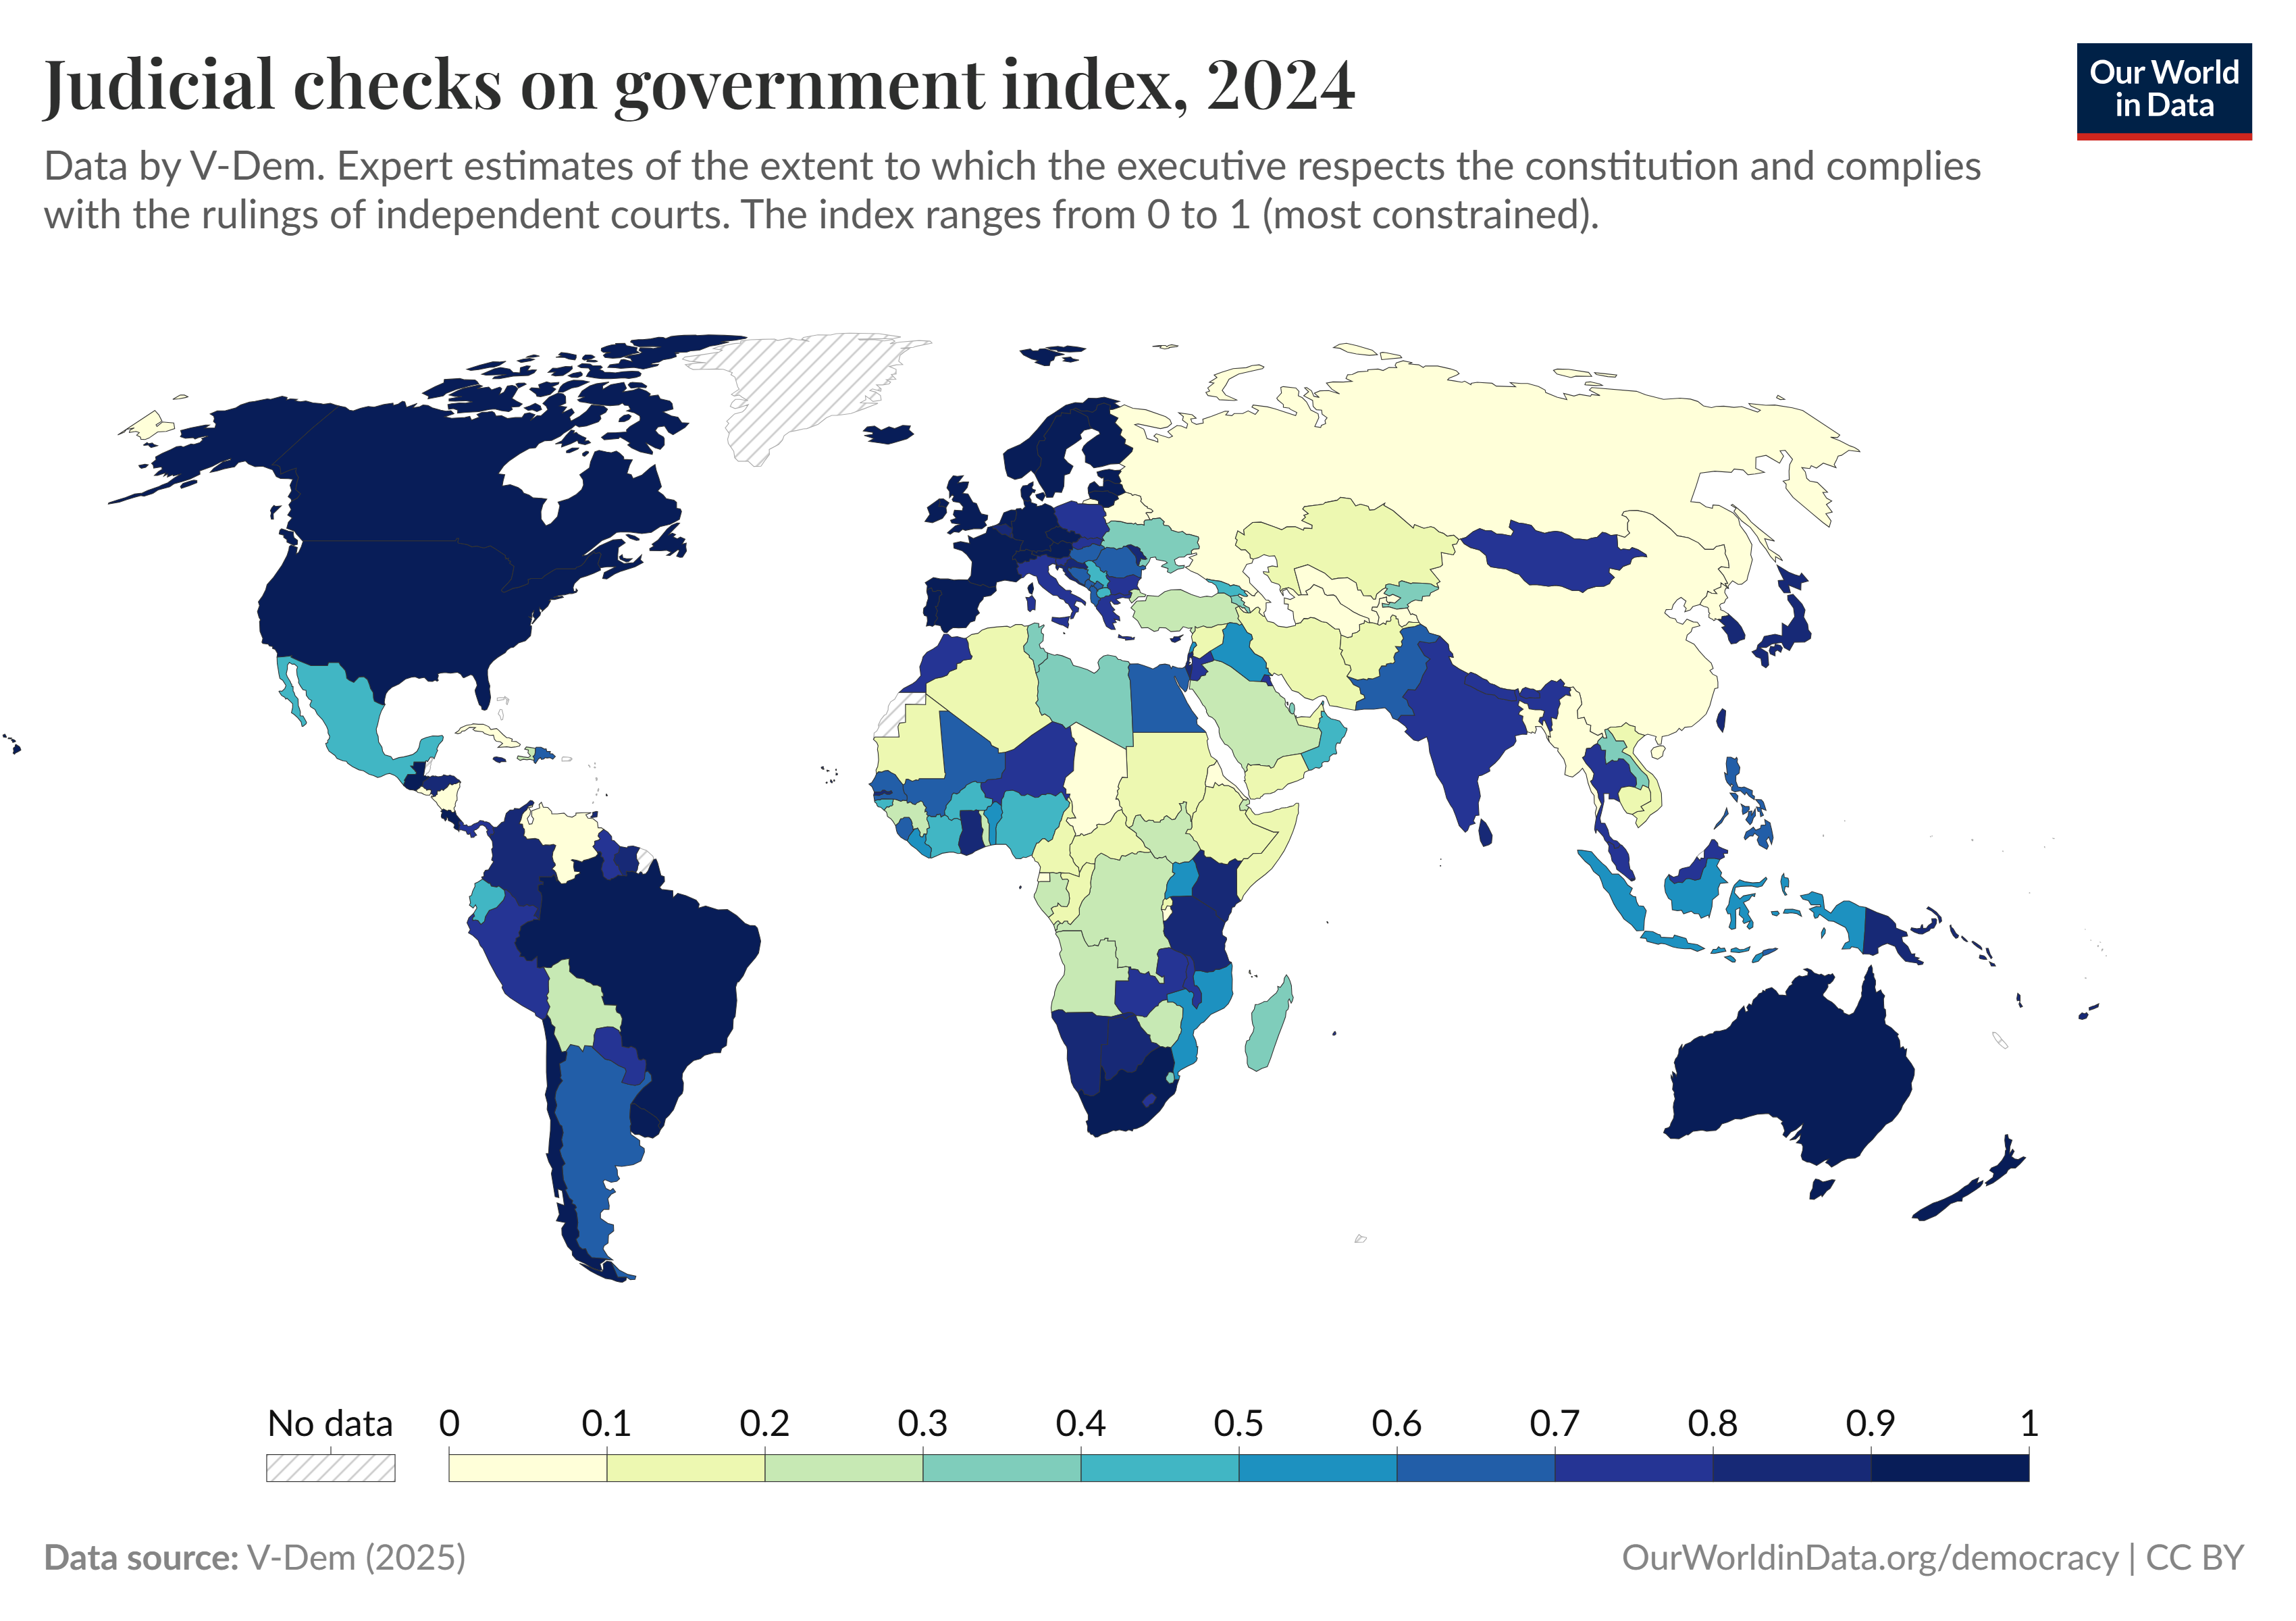
\includegraphics[width=1\linewidth]{figuras/judicial-constraints-on-the-executive-index.png}
	\label{fig:judicial-constraints-on-the-executive-index}
	\footnotesize{Fonte: \cite{jus_constraints_on_gov}.}
\end{figure}

Nota-se como o Poder Judiciário tem pouquíssimo controle sobre o Poder Executivo na em uma quantidade grande de países. A figura detalha o referido controle judicial no Brasil desde 1822 até 2024.

\begin{figure}[H]
    \centering
    \caption{Índice de controle judicial sobre o Poder Executivo no Brasil (1822-2024)}
    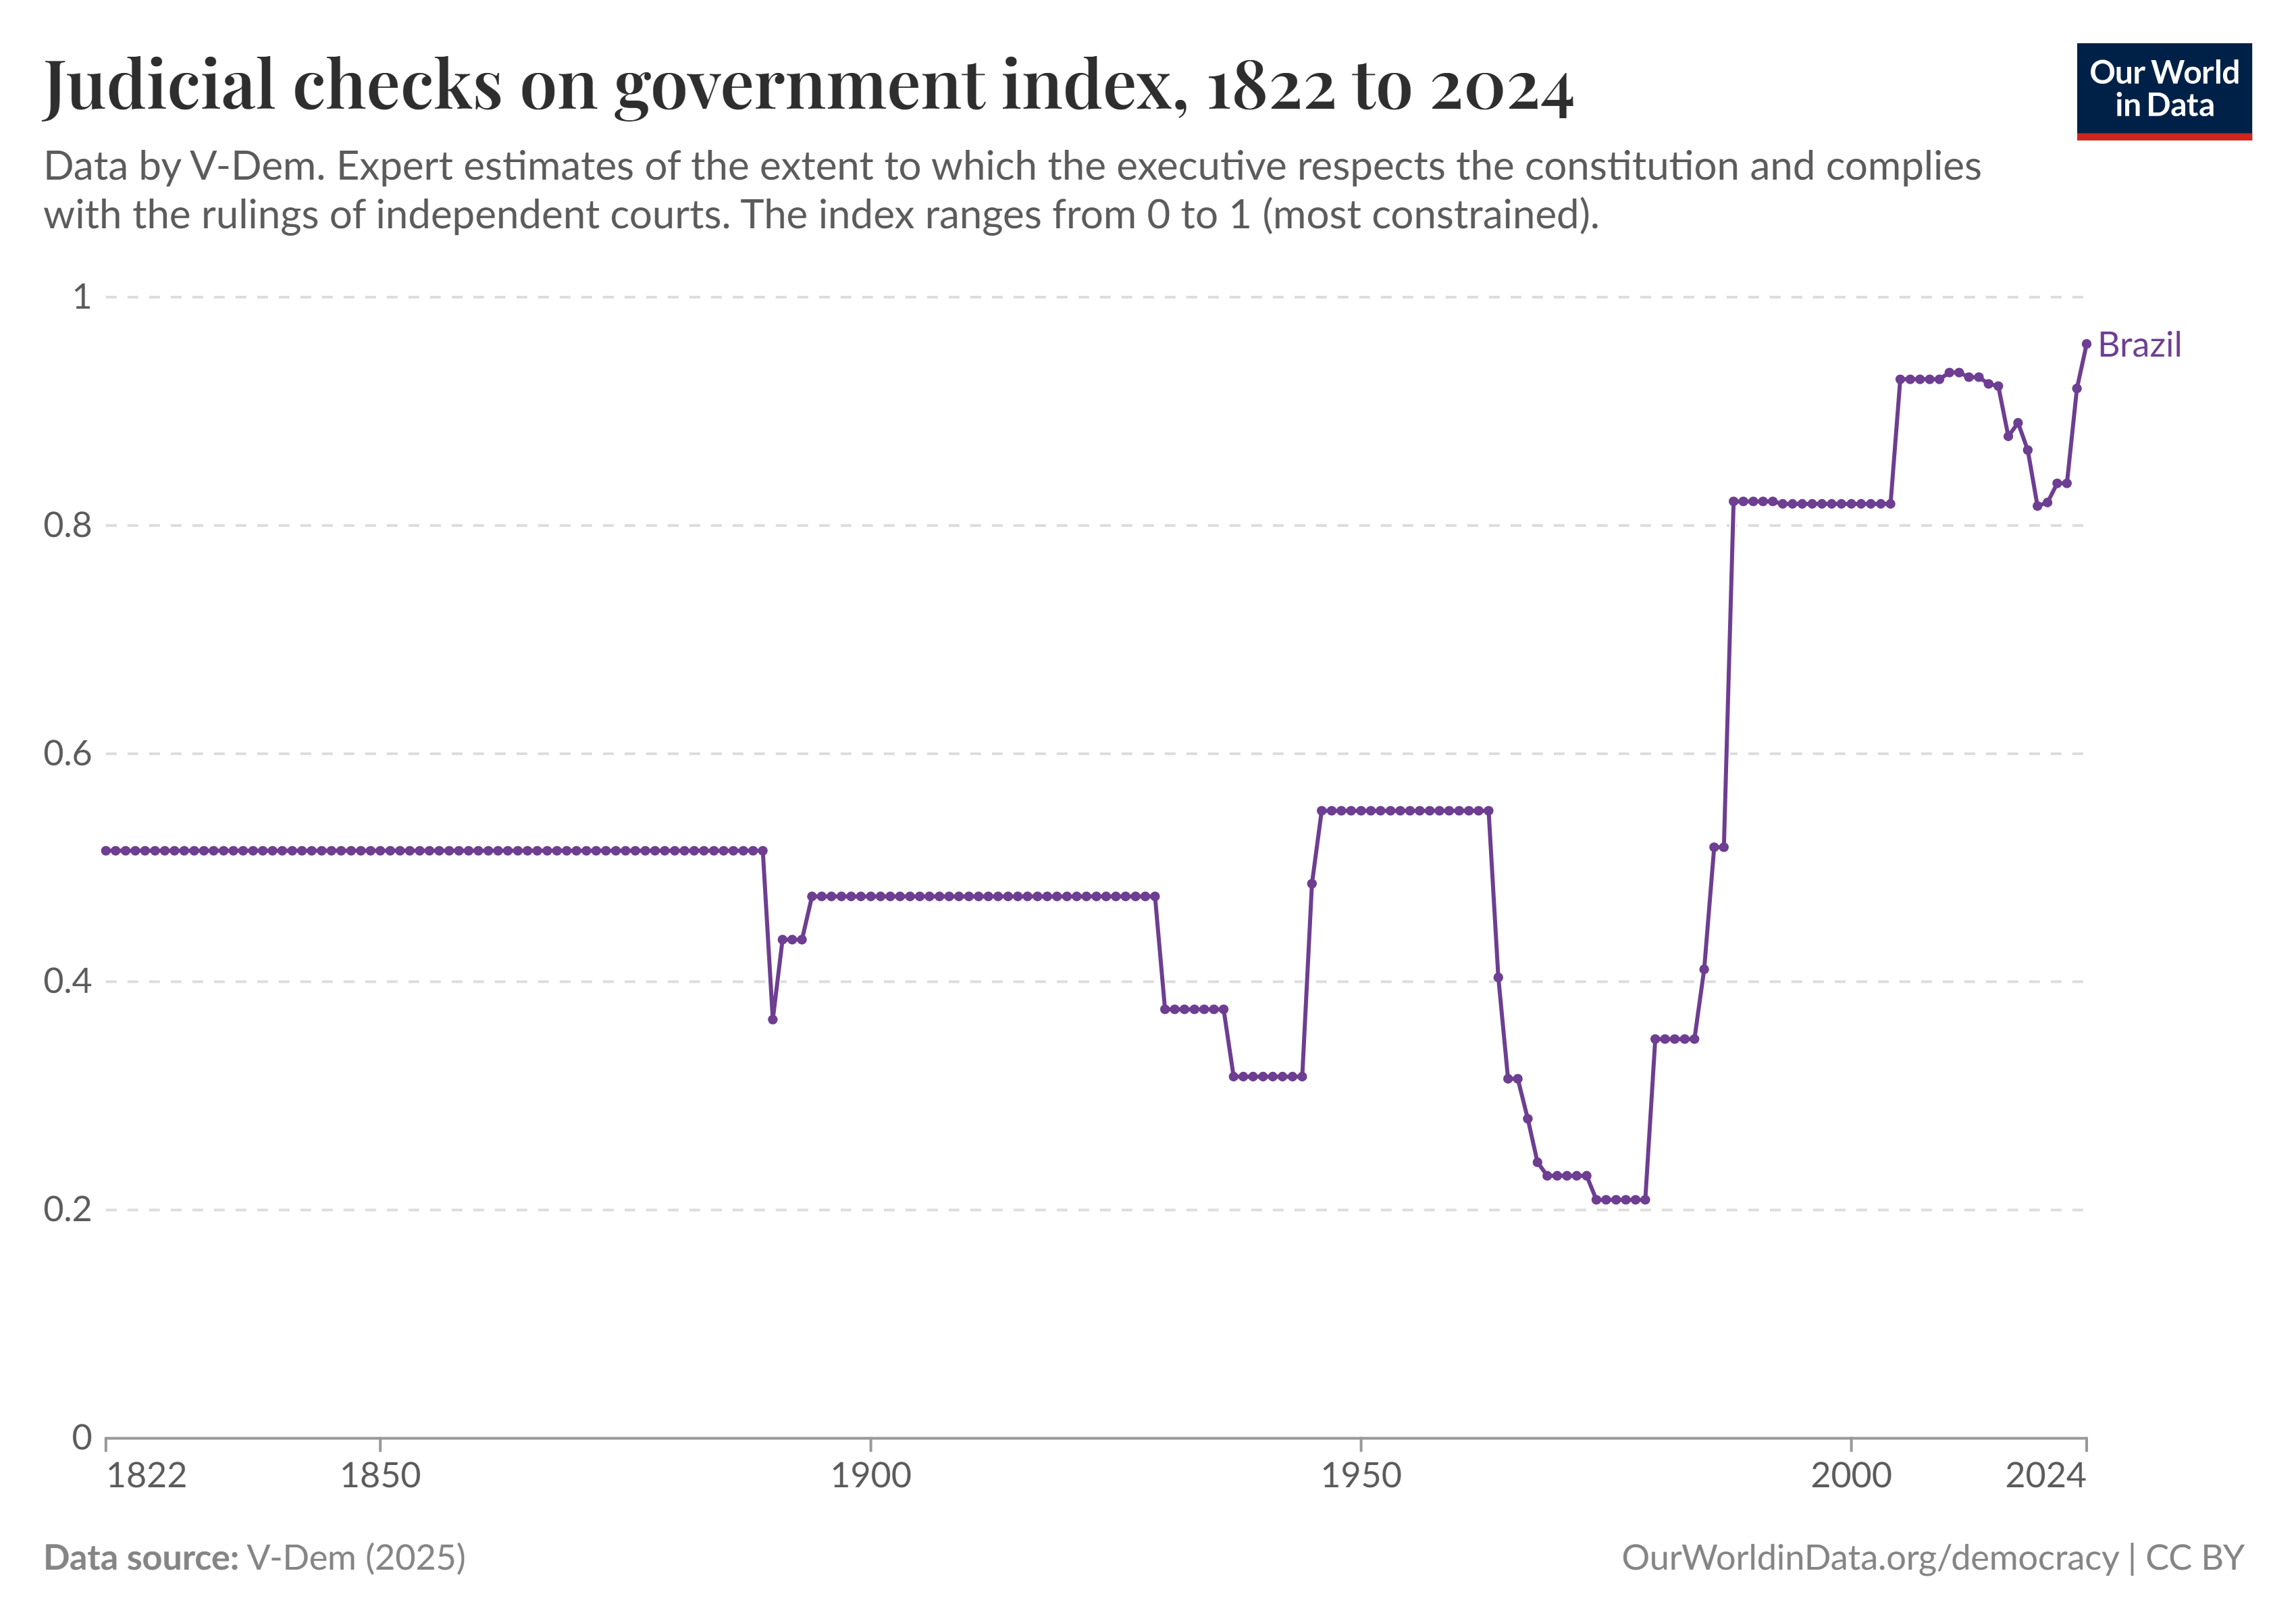
\includegraphics[width=1\linewidth]{figuras/judicial-constraints-on-the-executive-index-brazil.png}
    \label{fig:judicial-constraints-on-the-executive-index-brazil}
    \footnotesize{Fonte: \cite{jus_constraints_on_gov}.}
\end{figure}

No tocante a figura \ref{fig:judicial-constraints-on-the-executive-index-brazil}, nota-se como a democracia melhorou os índices do Brasil. Em 2024, o Brasil quase atingiu o valor máximo - 0,96 - enquanto a média mundial foi 0,664. Apenas 31 países de 193 - equivalente a 16\% do total - alcançaram uma pontuação de, no mínimo, 0,9 de 1,0 até o máximo.

A figura \ref{fig:quartis_controle_jus_sobre_gov} contém o Índice de controle judicial sobre o Poder Executivo.

\begin{figure}[H]
    \centering
    \caption{Índice de controle judicial sobre o Poder Executivo}
    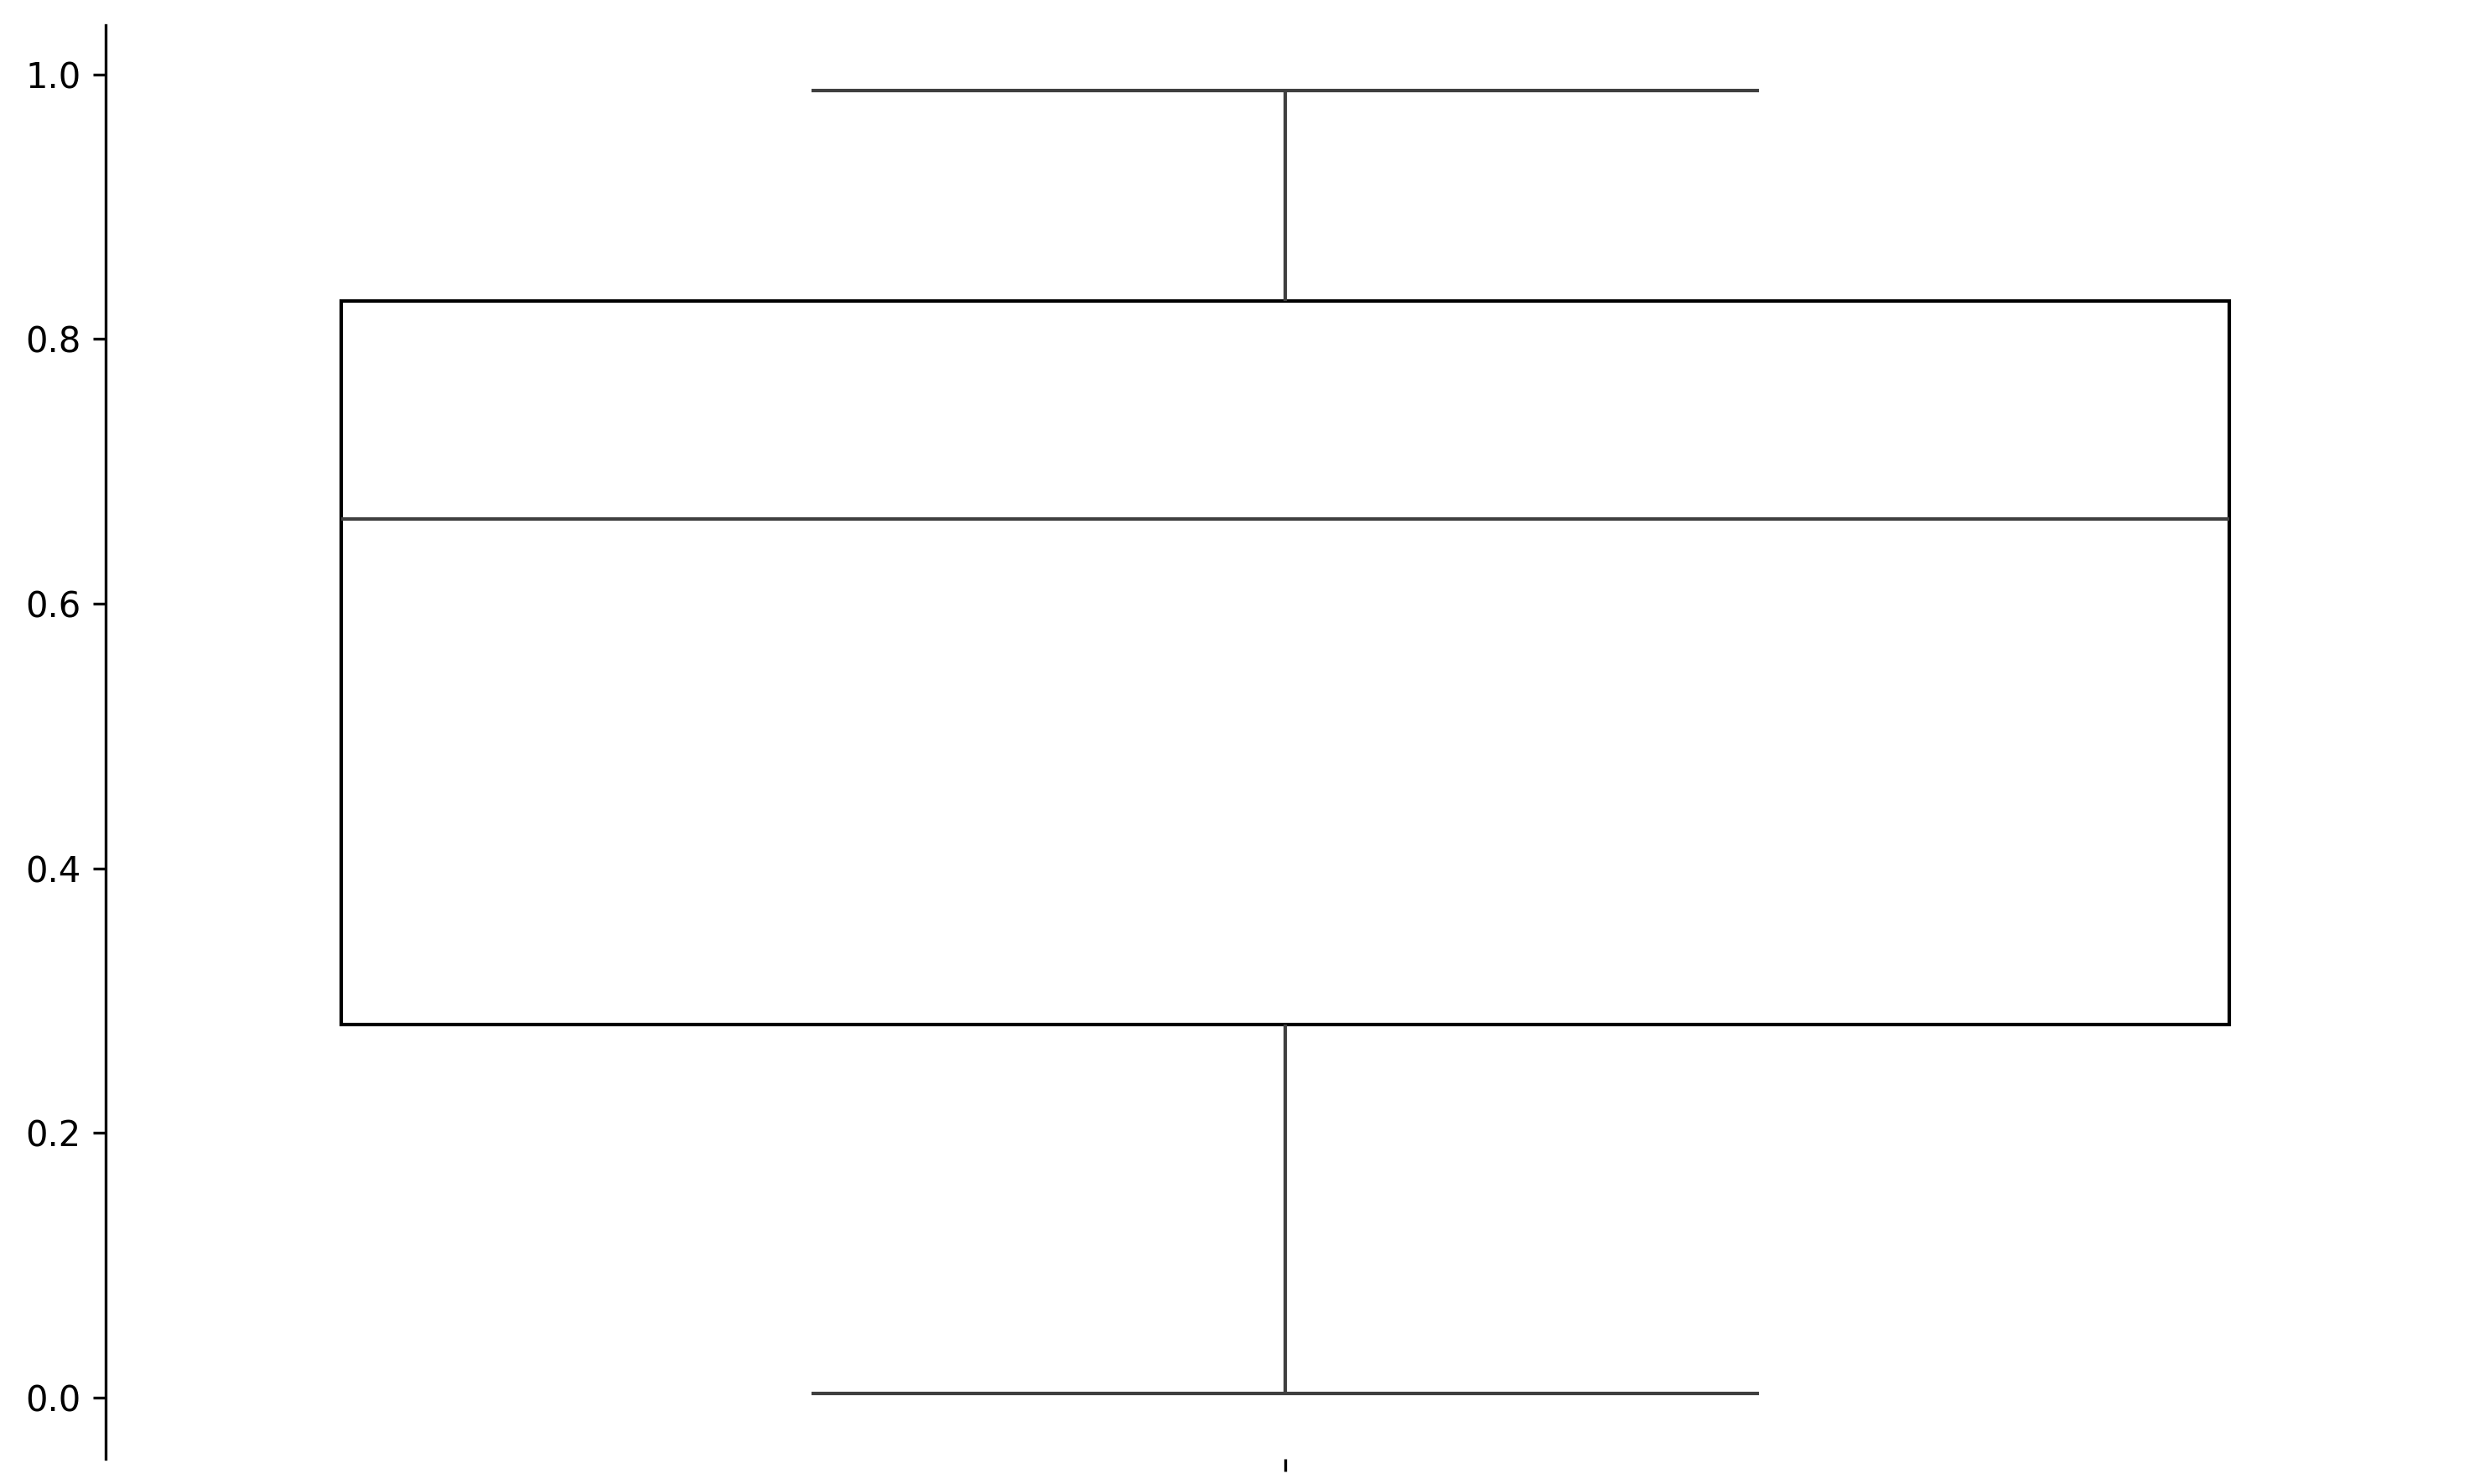
\includegraphics[width=1\linewidth]{figuras/quartis_controle_jus_sobre_gov.png}
    \label{fig:quartis_controle_jus_sobre_gov}
    \footnotesize{Fonte: elaboração própia baseada em \cite{jus_constraints_on_gov}.}
\end{figure}

A figura \ref{fig:quartis_controle_jus_sobre_gov}, que mostra a distribuição do índice de controle judicial sobre o Poder Executivo, ilustra que no ano de 2024 teve um valor mínimo de 0,003 e um máximo de 0,988. A média dos dados foi de 0,664. Além disso, 25\% dos valores ficaram abaixo de 0,282 (1º quartil), enquanto 75\% dos valores foram inferiores a 0,829 (3º quartil).

A figura \ref{fig:judicial-corruption-score} mostra os índices globais de corrupção judiciária.

\begin{figure}[H]
	\centering
	\caption{Pontuação de corrupção judicial no mundo em 2024}
	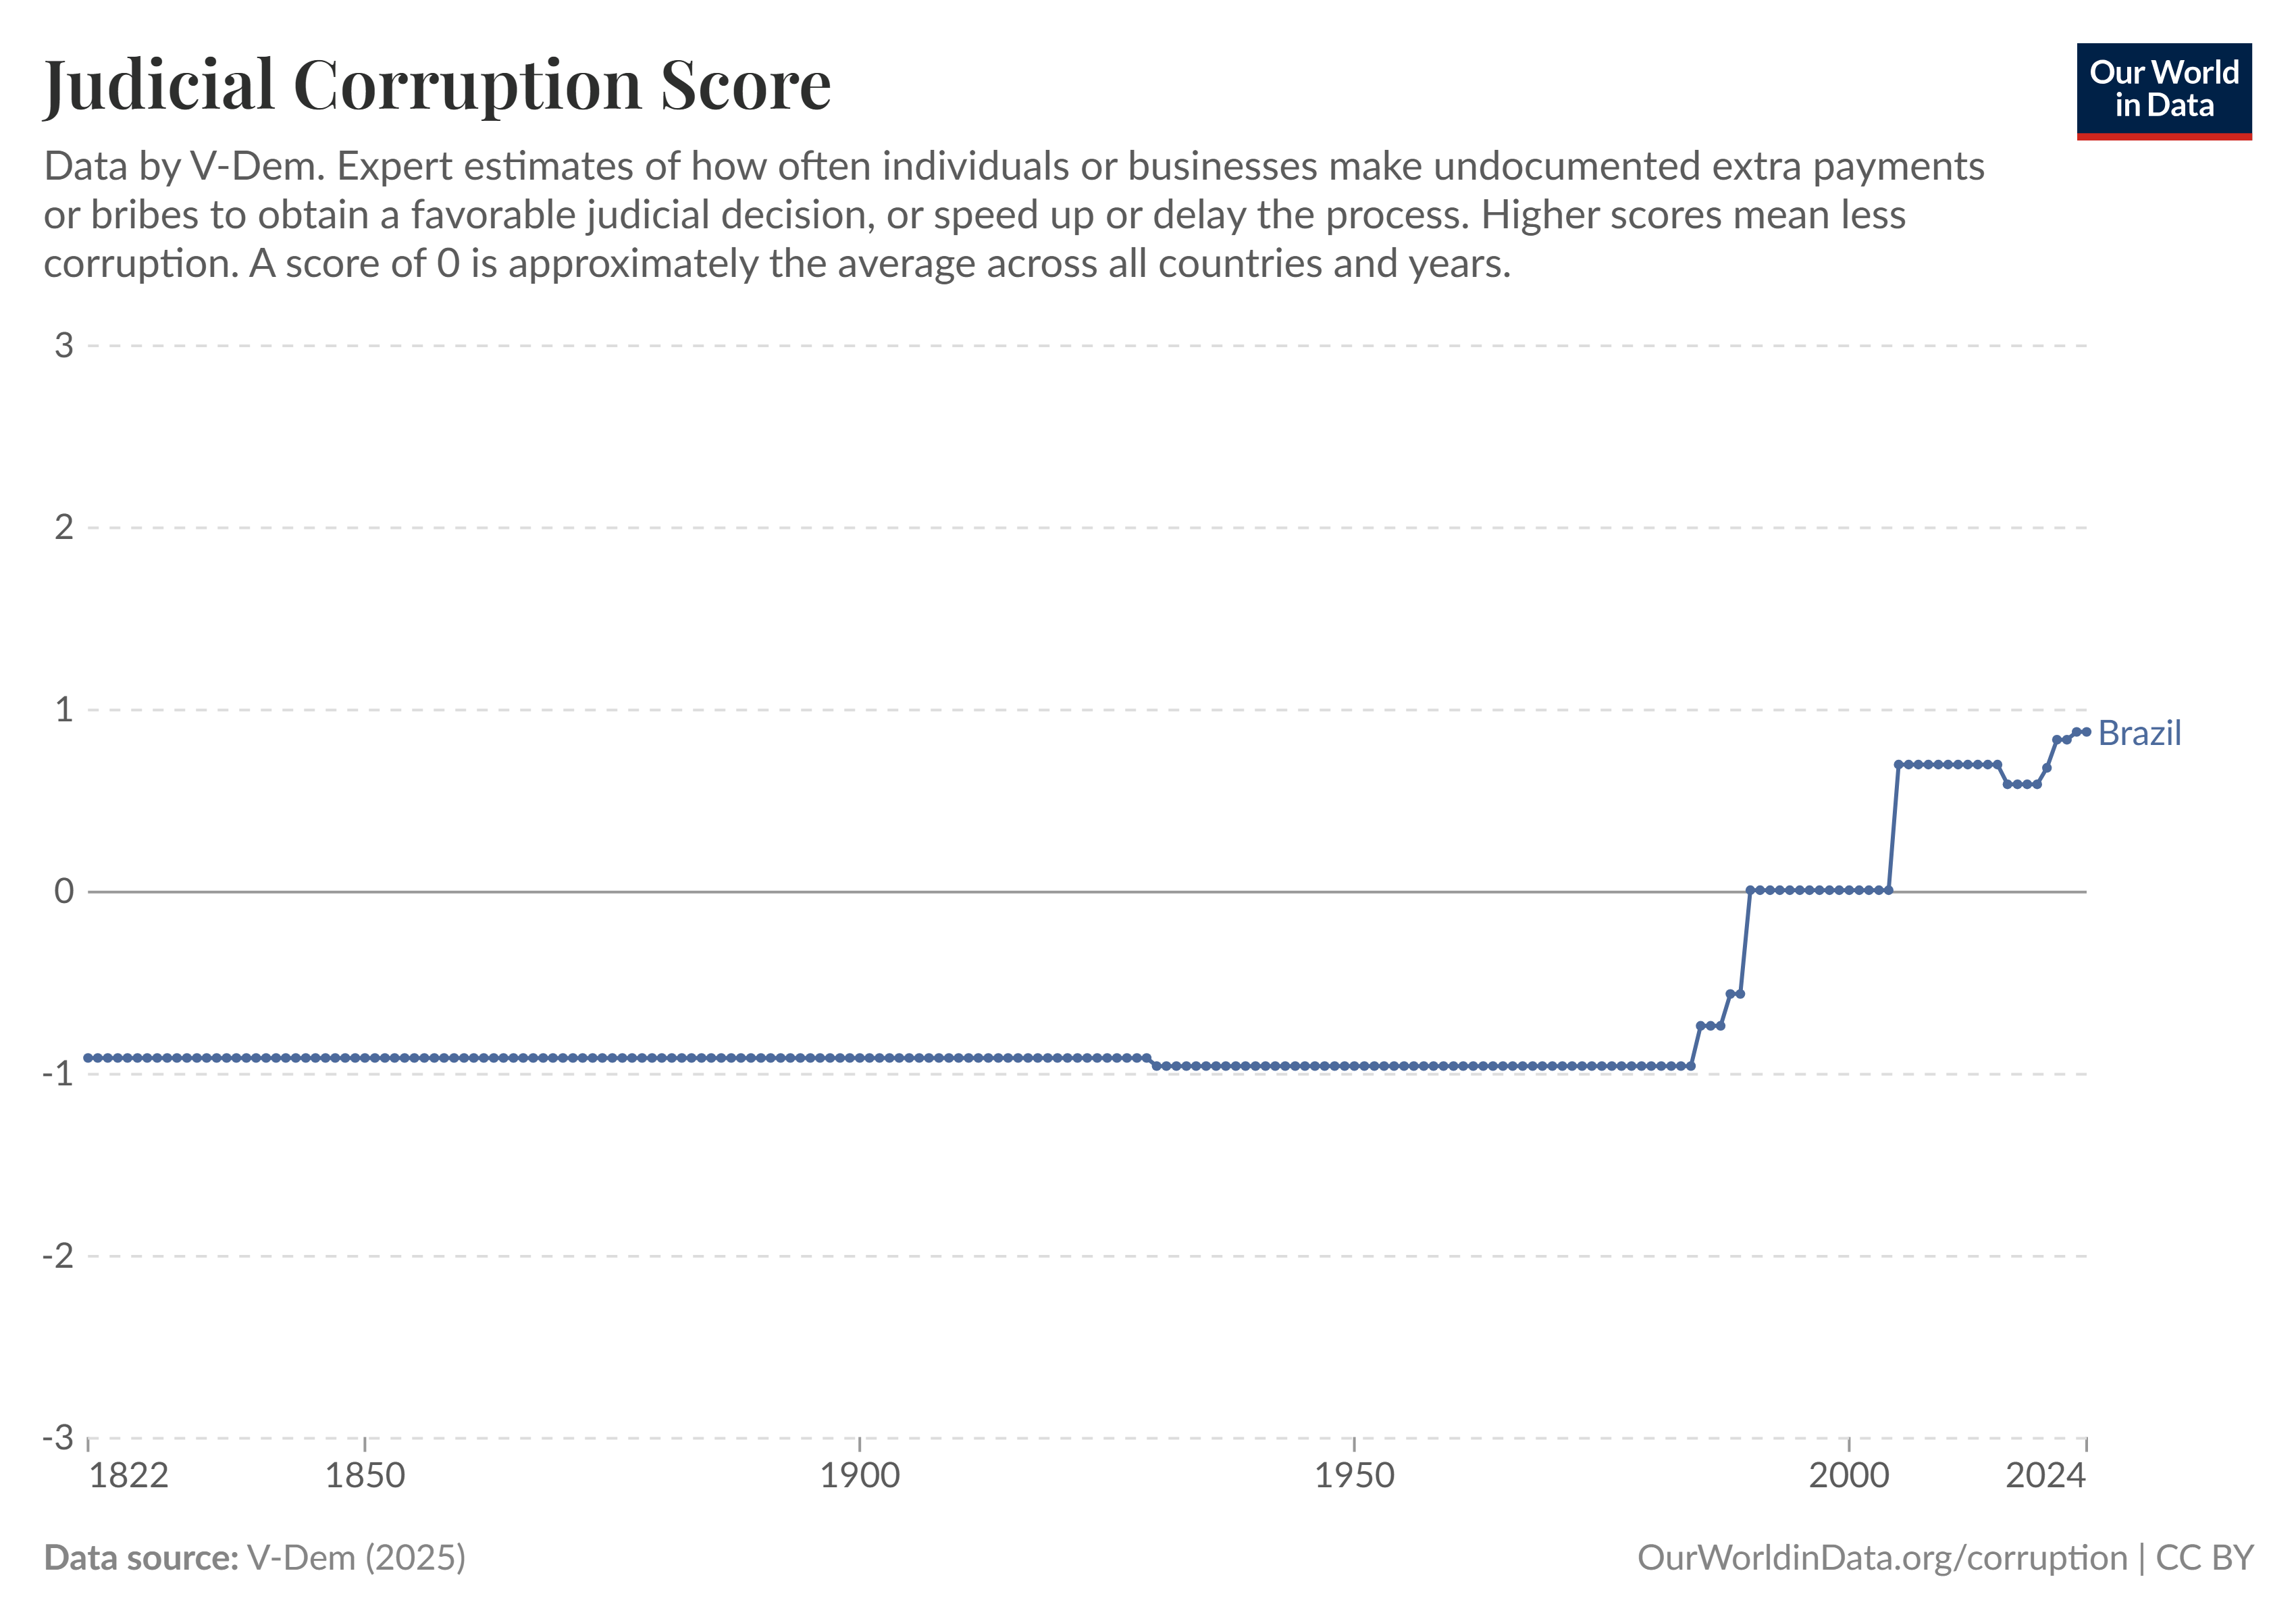
\includegraphics[width=1\linewidth]{figuras/judicial-corruption-score.png}
	\label{fig:judicial-corruption-score}
	\footnotesize{Fonte: \cite{judicial-corruption-score}.}
\end{figure}

Nota-se que uma quantidade grande de países tem alta corrupção judiciária. A figura \ref{fig:judicial-corruption-score} complementa a anterior ao especificar a situação histórica do Brasil (desde 1822 até 2024).

A figura \ref{fig:judicial-corruption-score-brazil} mostra como o Brasil melhorou o aspecto da corrupção judiciária. 

\begin{figure}[H]
    \centering
    \caption{Pontuação de corrupção judicial no Brasil (1822-2024)}
    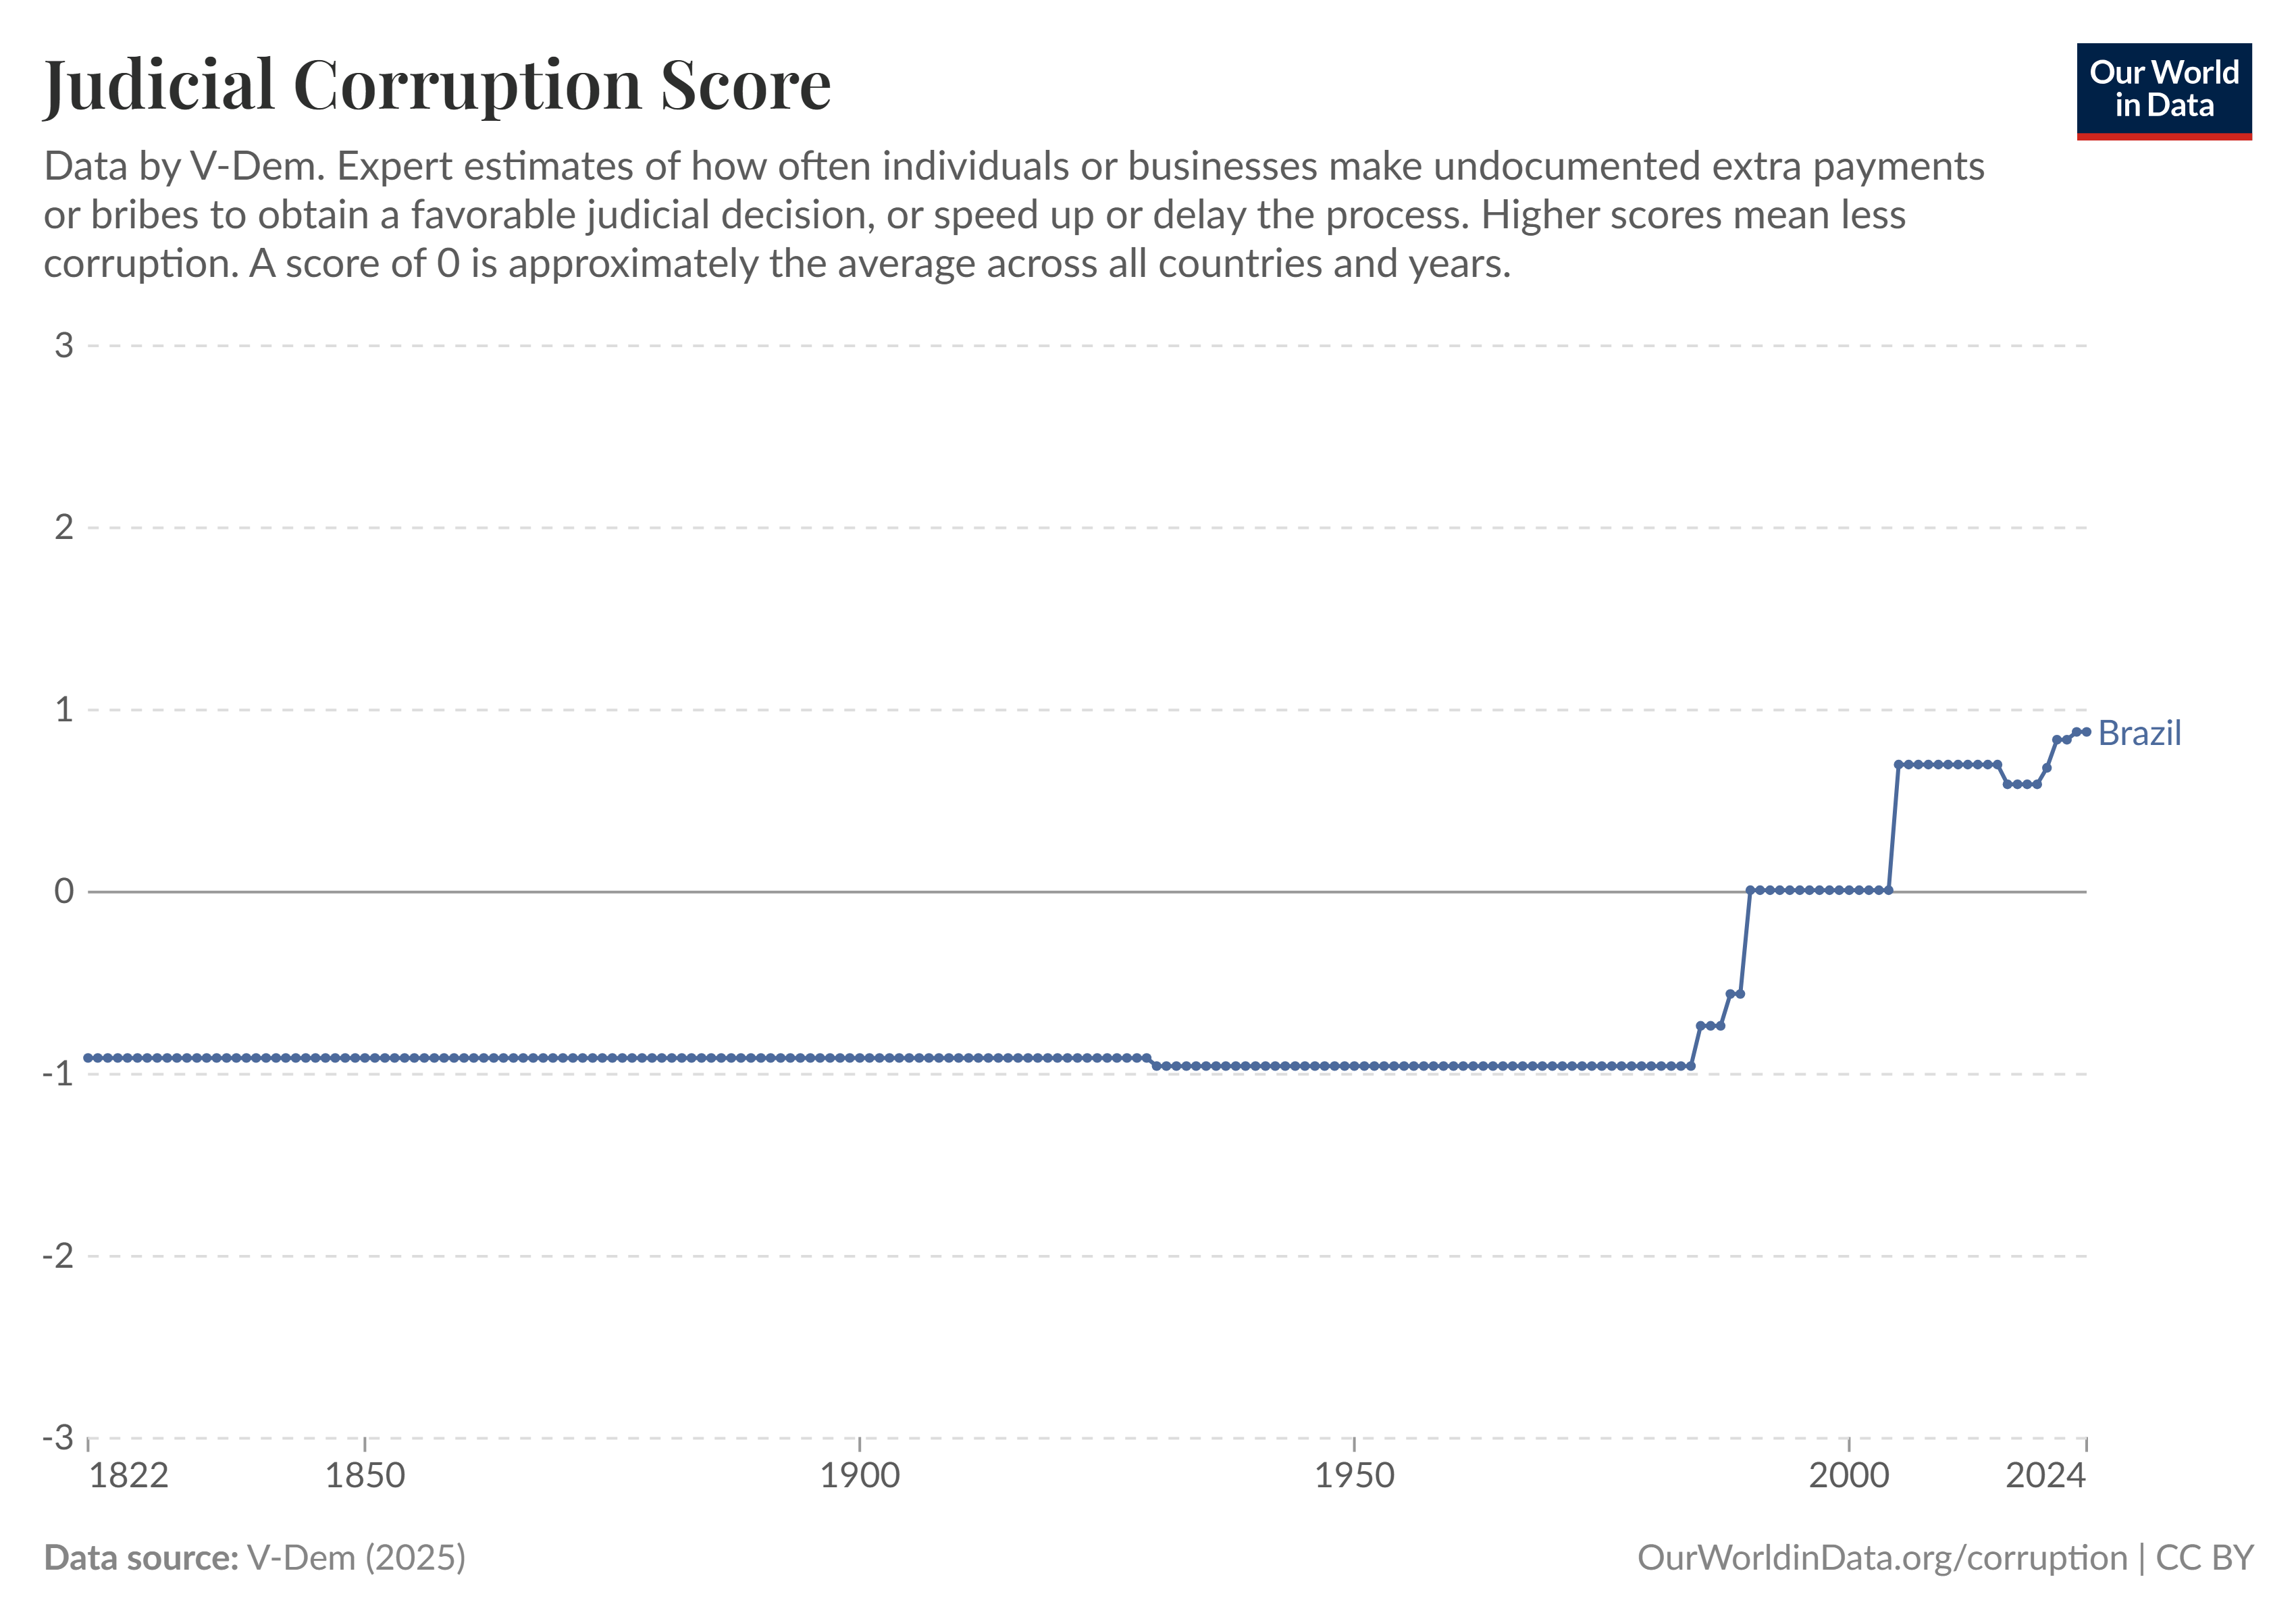
\includegraphics[width=1\linewidth]{figuras/judicial-corruption-score-brazil.png}
    \label{fig:judicial-corruption-score-brazil}
    \footnotesize{Fonte: \cite{judicial-corruption-score}.}
\end{figure}

Durante décadas, o Brasil ficou na faixa -1, alcançando 0 até 0,88. A atual pontuação do Brasil não está entre as melhores, pois ainda há as pontuações 2 e 3. No entanto, como a média mundial foi 0,249, o Brasil está acima da média mundial, porém o país foi superado por 66 países, cujas pontuações superaram 0,88. A quantidade de países que atingiu, no mínimo, 1 foi 29,84\%; no tocante a pontuação 2, foi 12\%; e por fim, 3 foi 3\% e nenhum atingiu 4 (valor máximo).

De maneira complementar, a figura \ref{fig:quartis_corrupcao_judiciaria} contém o gráfico de caixa da pontuação de corrupção judicial.

\begin{figure}[H]
    \centering
    \caption{Gráfico da caixa: corrupção judiciária}
    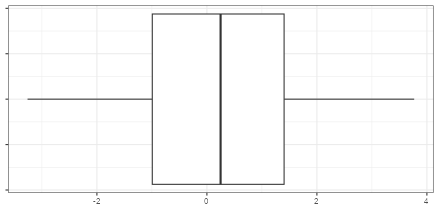
\includegraphics[width=1\linewidth]{figuras/quartis_corrupcao_judiciaria.png}
    \label{fig:quartis_corrupcao_judiciaria}
    \footnotesize{Fonte: elaboração própria baseada em \cite{judicial-corruption-score}.}
\end{figure}

A figura \ref{fig:quartis_corrupcao_judiciaria}, que mostra a distribuição do índice de corrupção judiciária, ilustra que no ano de 2024 teve um valor mínimo de -3,2610 e um máximo de 3,7690. A média dos dados foi de 0,2490. Além disso, 25\% dos valores ficaram abaixo de -0,9930 (1º quartil), enquanto 75\% dos valores foram inferiores a 1,4035 (3º quartil).

A figura \ref{fig:rule-of-law-index} mostra como a situação em 2024 do Estado de Direito no mundo.

\begin{figure}[H]
	\centering
	\caption{Estado de Direito no mundo em 2024}
	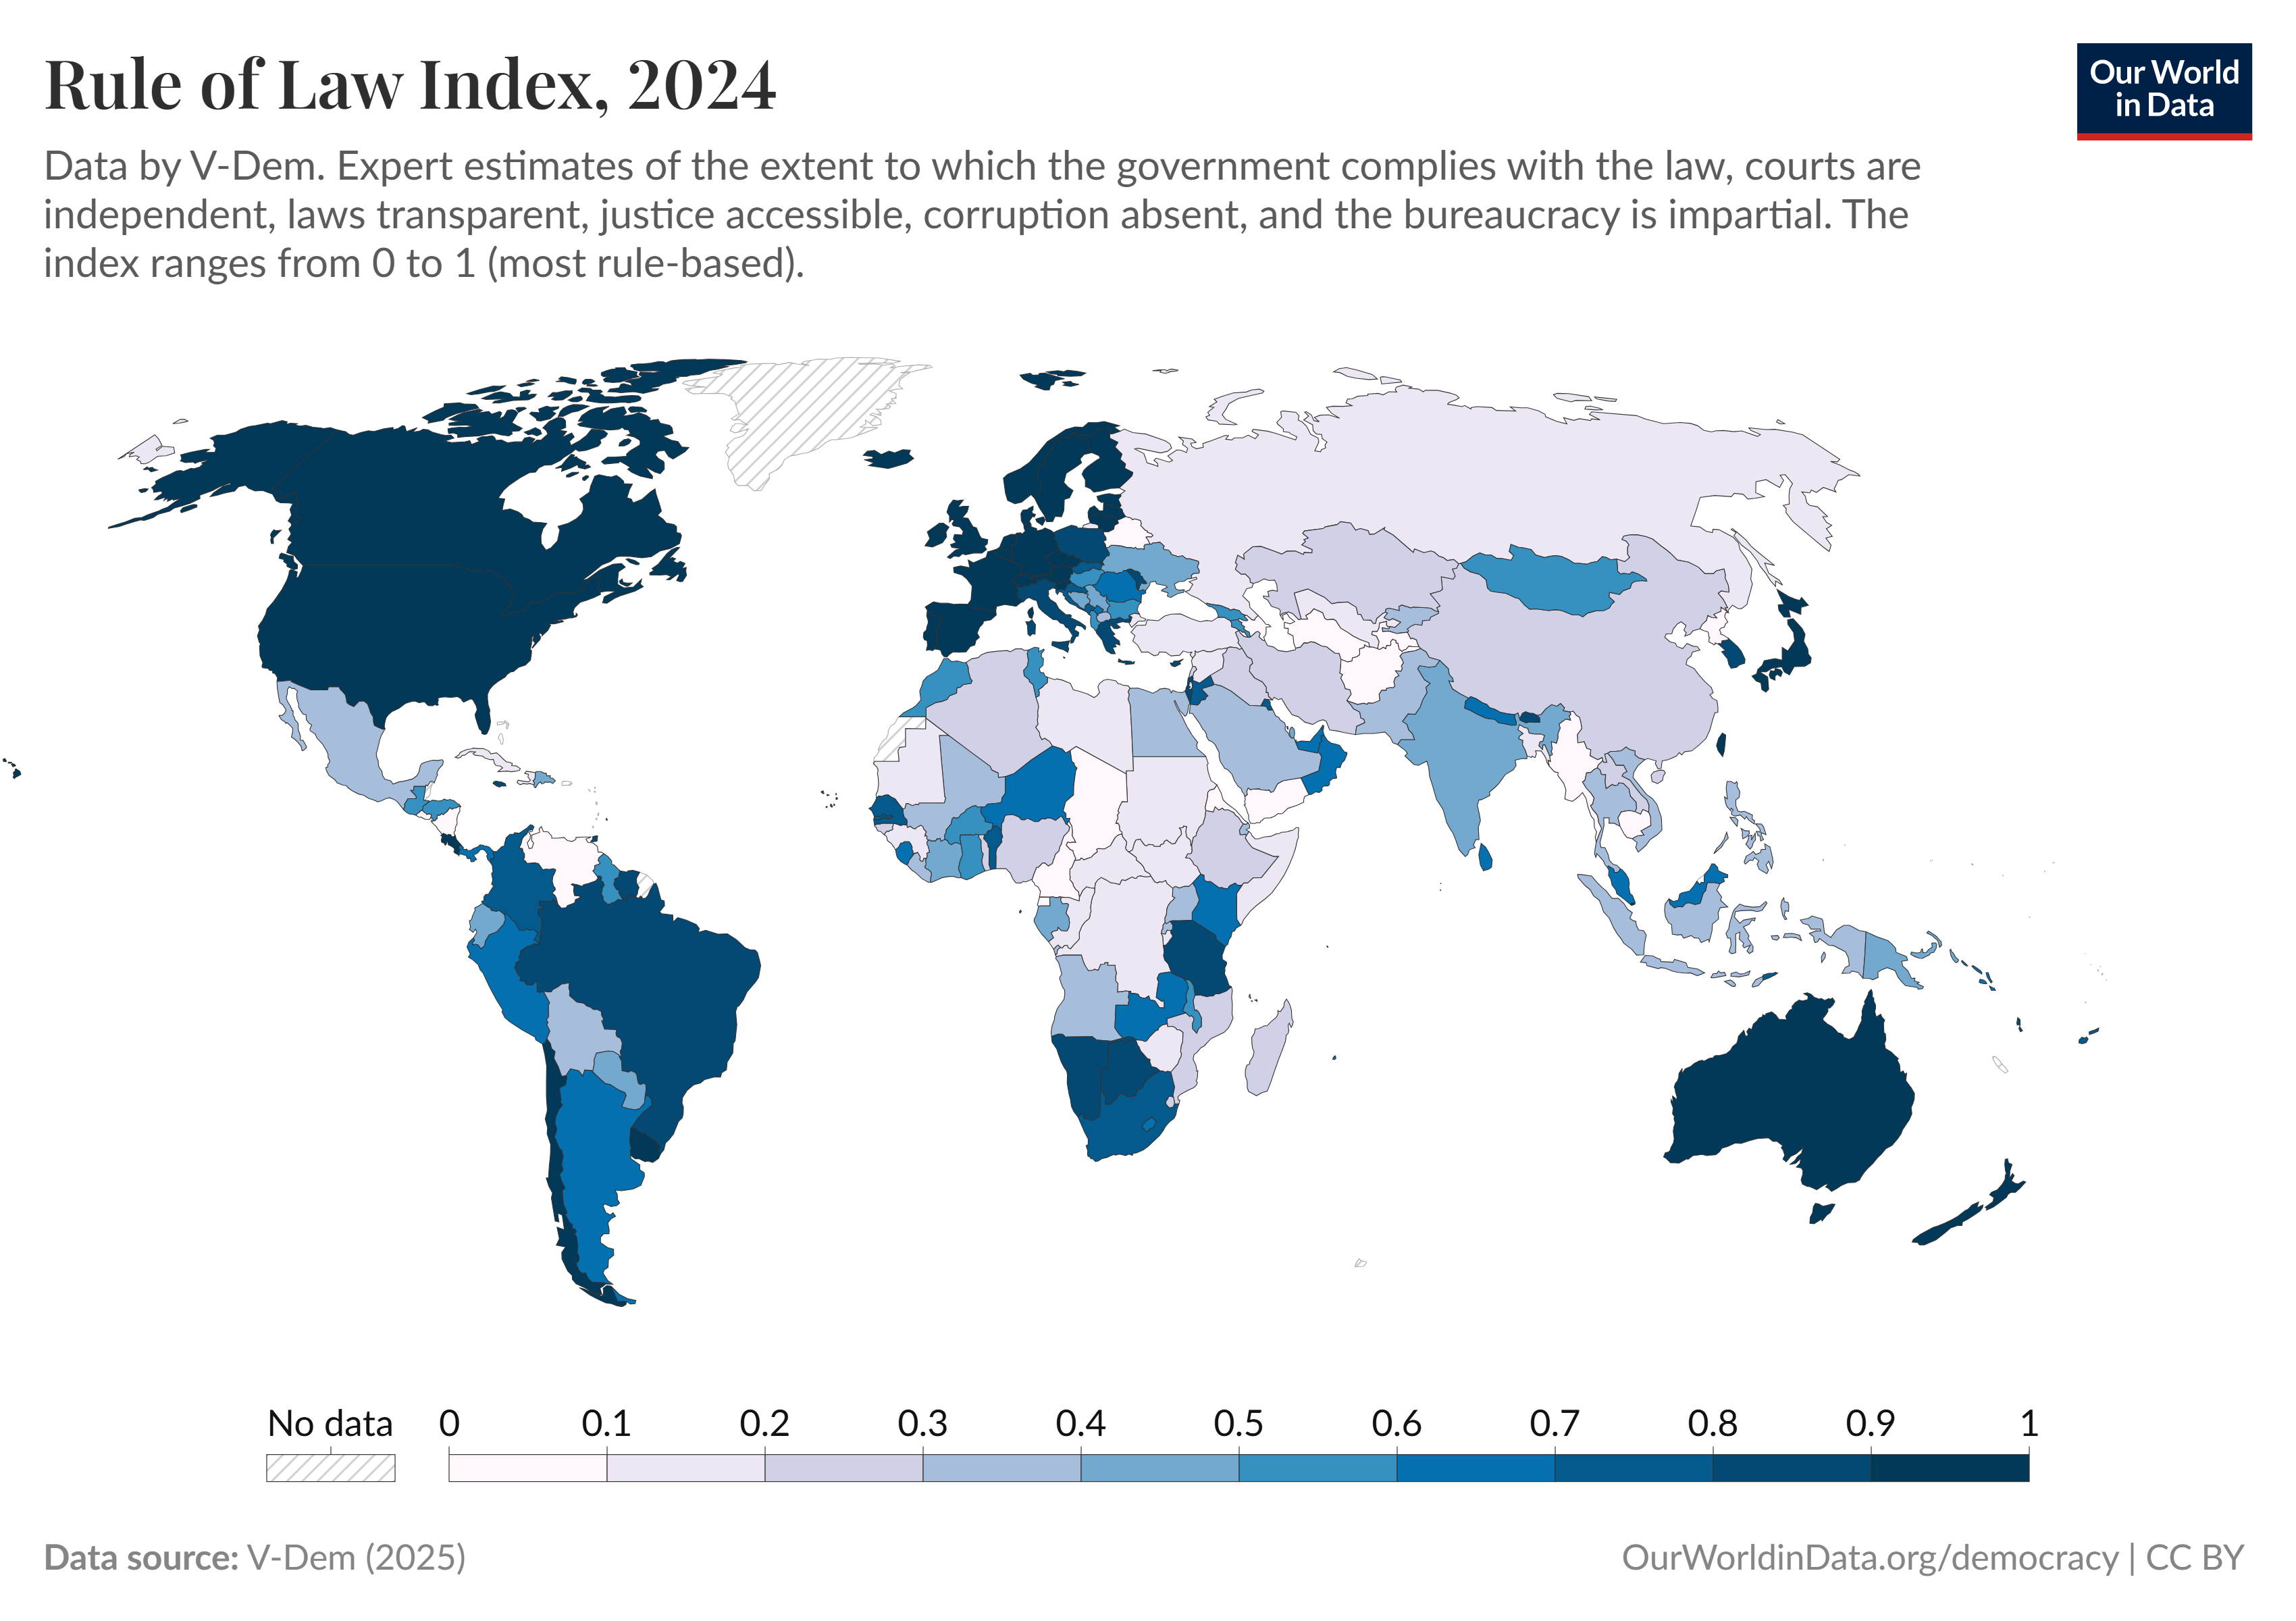
\includegraphics[width=1\linewidth]{figuras/rule-of-law-index.png}
	\label{fig:rule-of-law-index}
	\footnotesize{Fonte: \cite{rule-of-law-index}.}
\end{figure}

Nota-se como a instituição do Estado de Direito é muito fraco ou inexistente em muitos países do globo. De forma complementar a figura anterior, a figura \ref{fig:rule-of-law-index-brazil} mostra à situação histórica do Estado de Direito no Brasil (desde 1822 até 2024)

\begin{figure}[H]
	\centering
	\caption{Estado de Direito no Brasil (1822-2024)}
	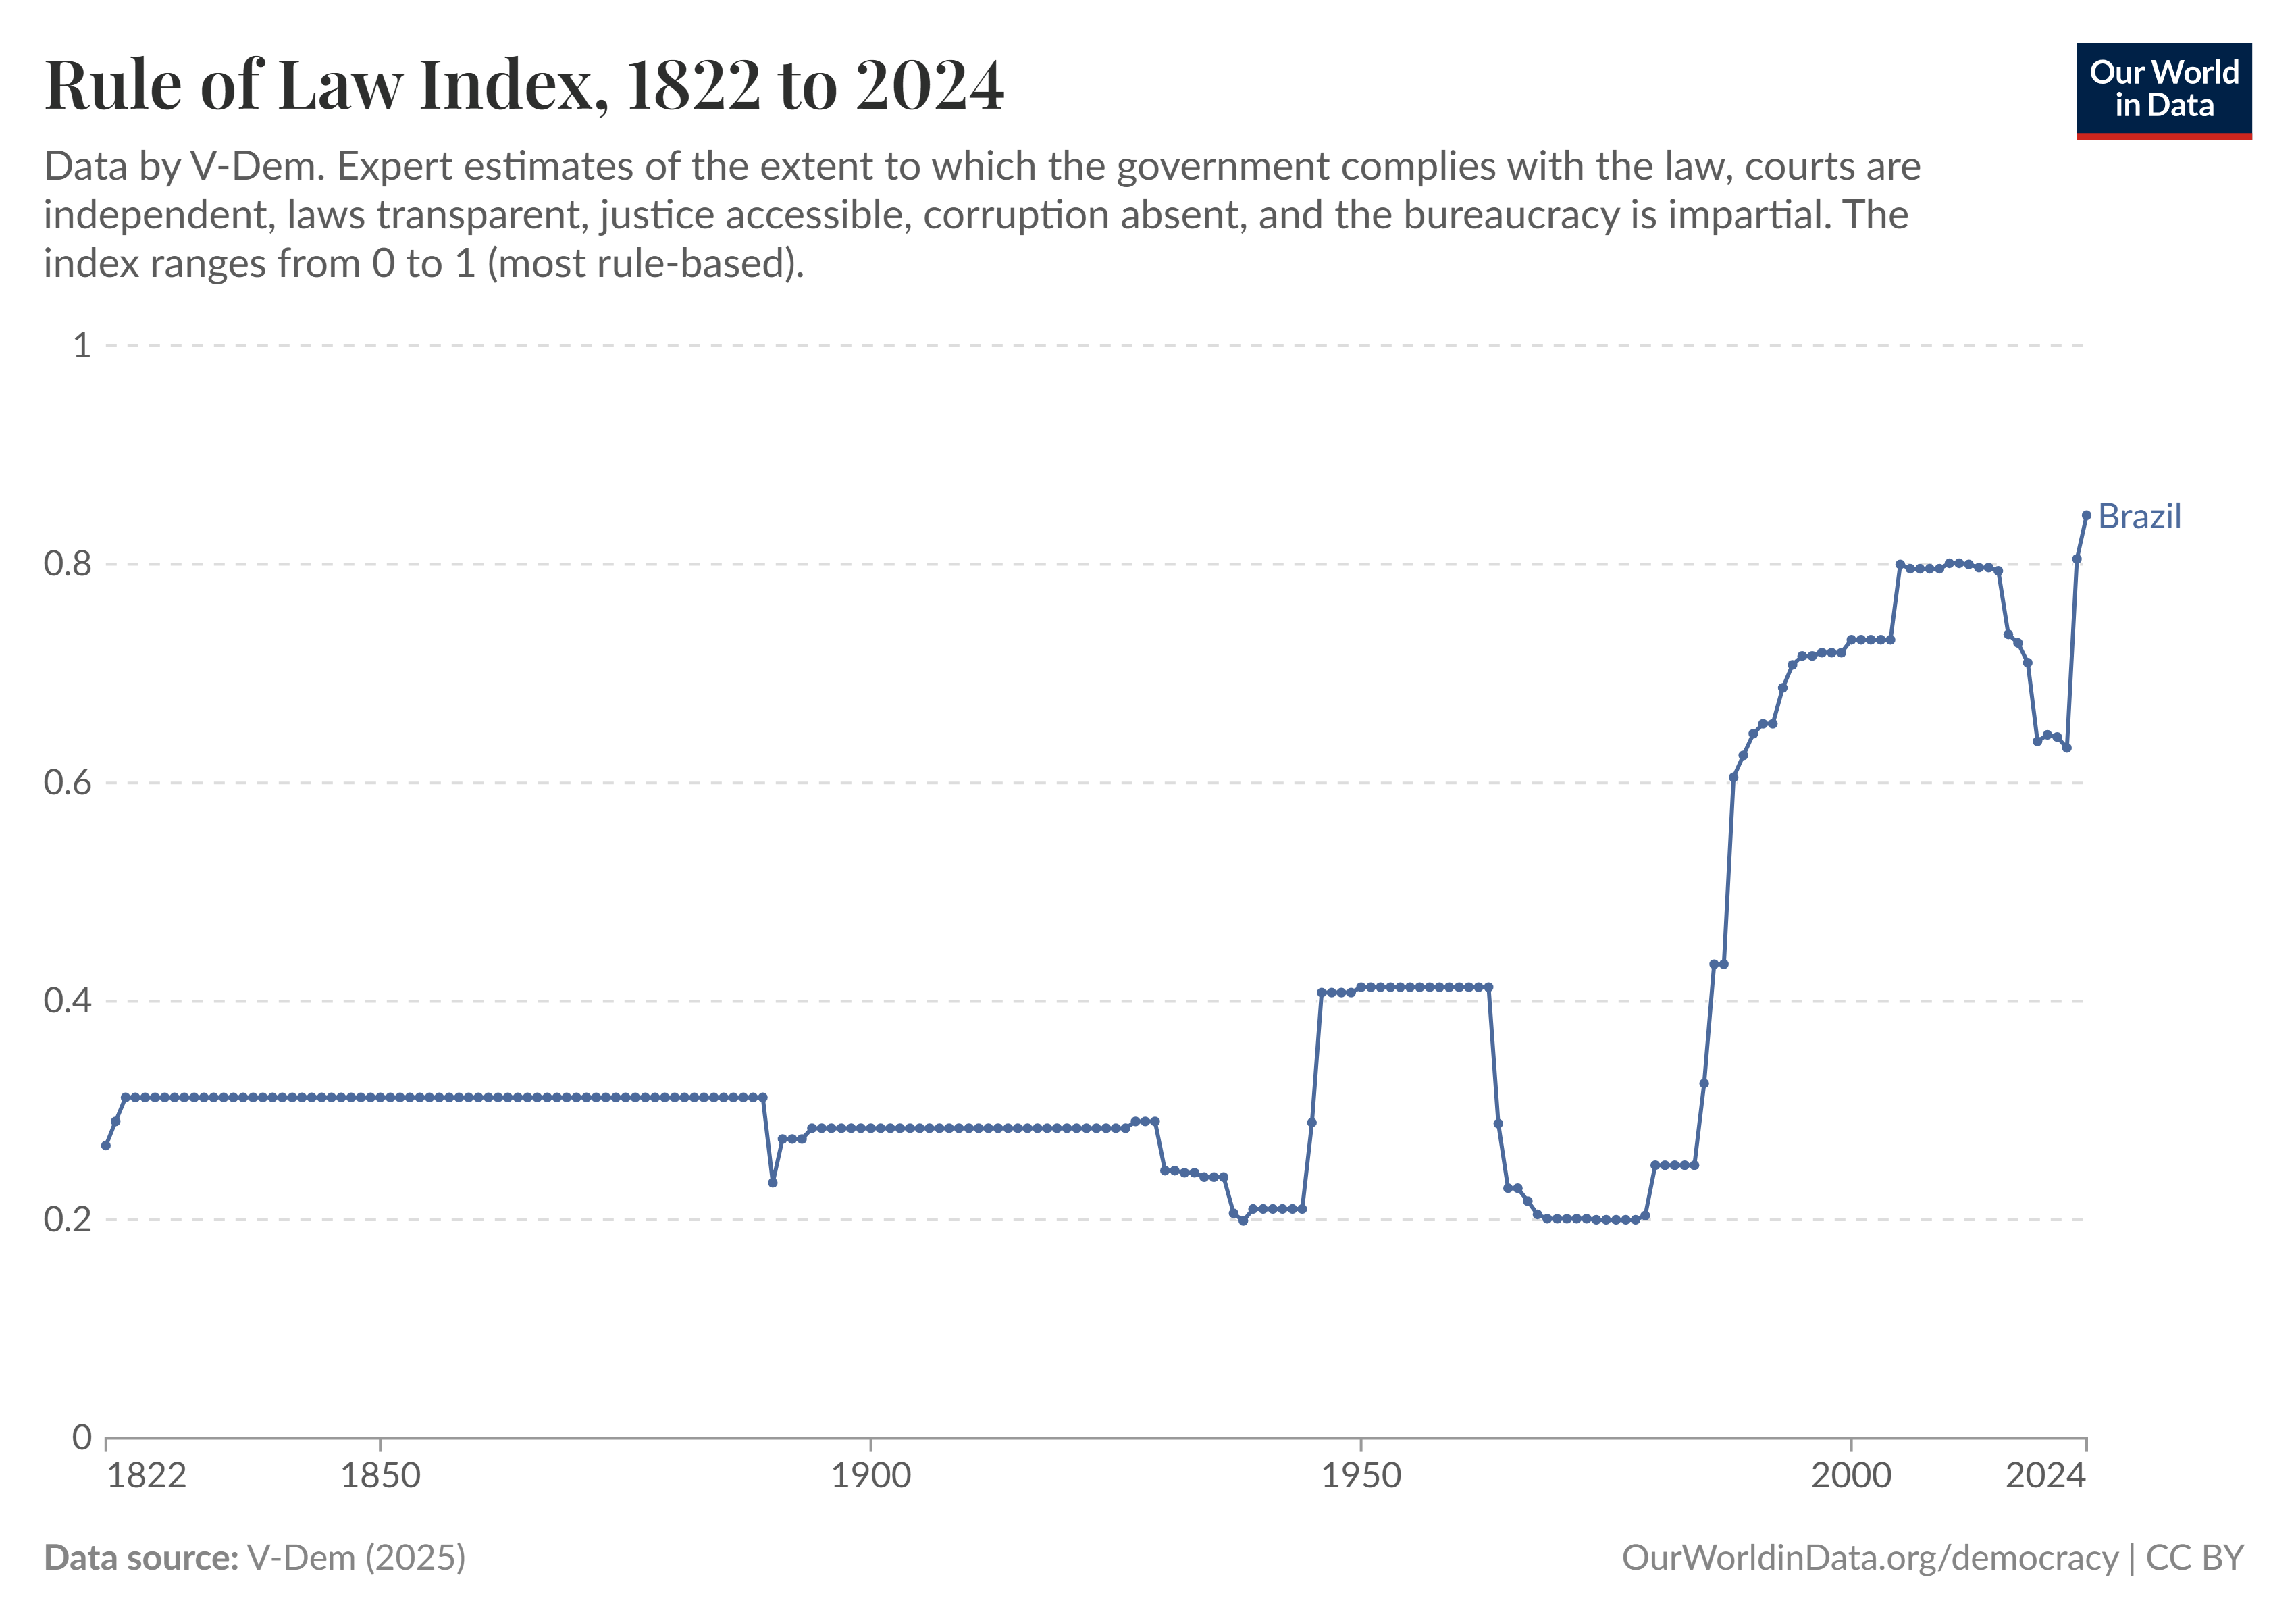
\includegraphics[width=1\linewidth]{figuras/rule-of-law-index-brazil.png}
	\label{fig:rule-of-law-index-brazil}
	\footnotesize{Fonte: \cite{rule-of-law-index}.}
\end{figure}

Nota-se como o Brasil evoluiu no aspecto do Estado de Direito. Durante mais de 100 anos (1822 até quase 1950), o Brasil ficou na baixa faixa 0,2-0,4, no entanto, atingiu o valor de 0,8 em 2023 e 0,84 em 2024 via políticas públicas que almejaram esse crescimento.

A figura \ref{fig:quartis_estado_direito} contém um gráfico de caixa.

\begin{figure}[H]
	\centering
	\caption{Gráfico da caixa: Estado de Direito}
	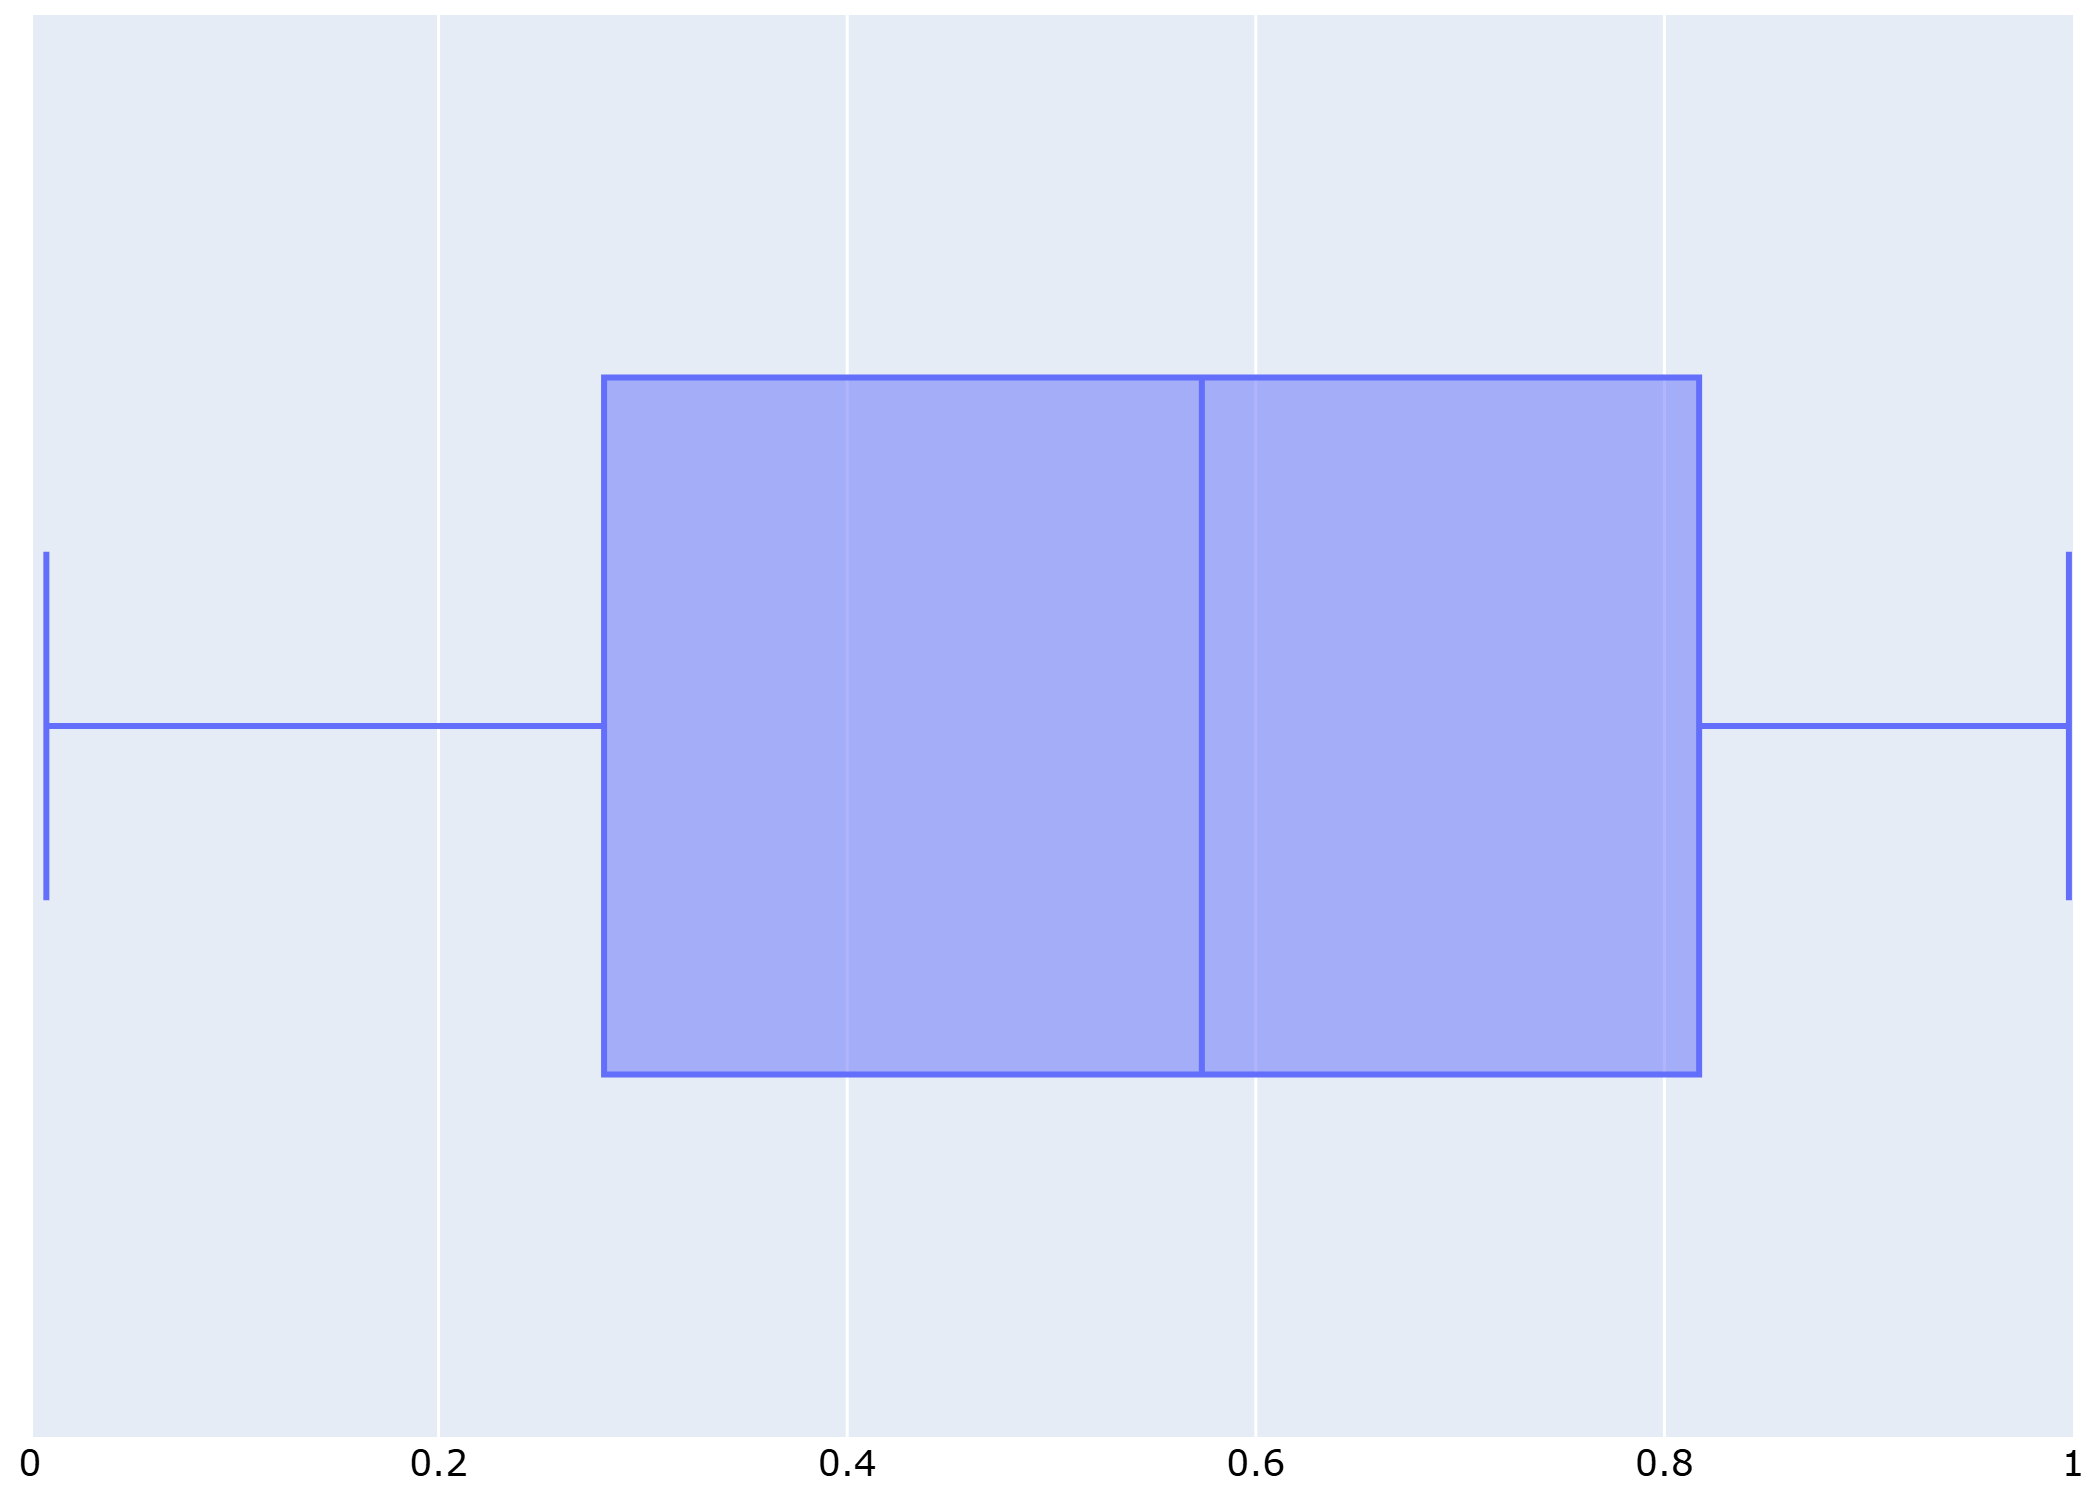
\includegraphics[width=1\linewidth]{figuras/quartis_estado_direito.png}
	\label{fig:quartis_estado_direito}
	\footnotesize{Fonte: elaboração própria baseada em \cite{rule-of-law-index}.}
\end{figure}

A figura \ref{fig:quartis_estado_direito}, que mostra a distribuição do índice de corrupção judiciária, ilustra que no ano de 2024 teve um valor mínimo de 0,008 e um máximo de 0,998. A média dos dados foi de 0,5736. Além disso, 25\% dos valores ficaram abaixo de 0,282 (1º quartil), enquanto 75\% dos valores foram inferiores a 0,816 (3º quartil).

Além da análise gráfica, estudou-se se há correlação entre o índice de democracia eleitoral com os índices de controle judicial sob o Poder Executivo, corrupção no Poder Judiciário, Estado de Direito e liberdades civis.

A figura \ref{fig:comparacao_democracia} contém um gráfico de barras que contêm os coeficientes de correlação das relações entre o índice de democracia eleitoral com os índices de controle judicial sob o Poder Executivo, corrupção no Poder Judiciário, Estado de Direito e liberdades civis.

\begin{figure}[H]
	\centering
	\caption{Coeficiente de correlação: índice de democracia eleitoral x índices de controle judicial sob o Poder Executivo, corrupção no Poder Judiciário, Estado de Direito e liberdades civis}
	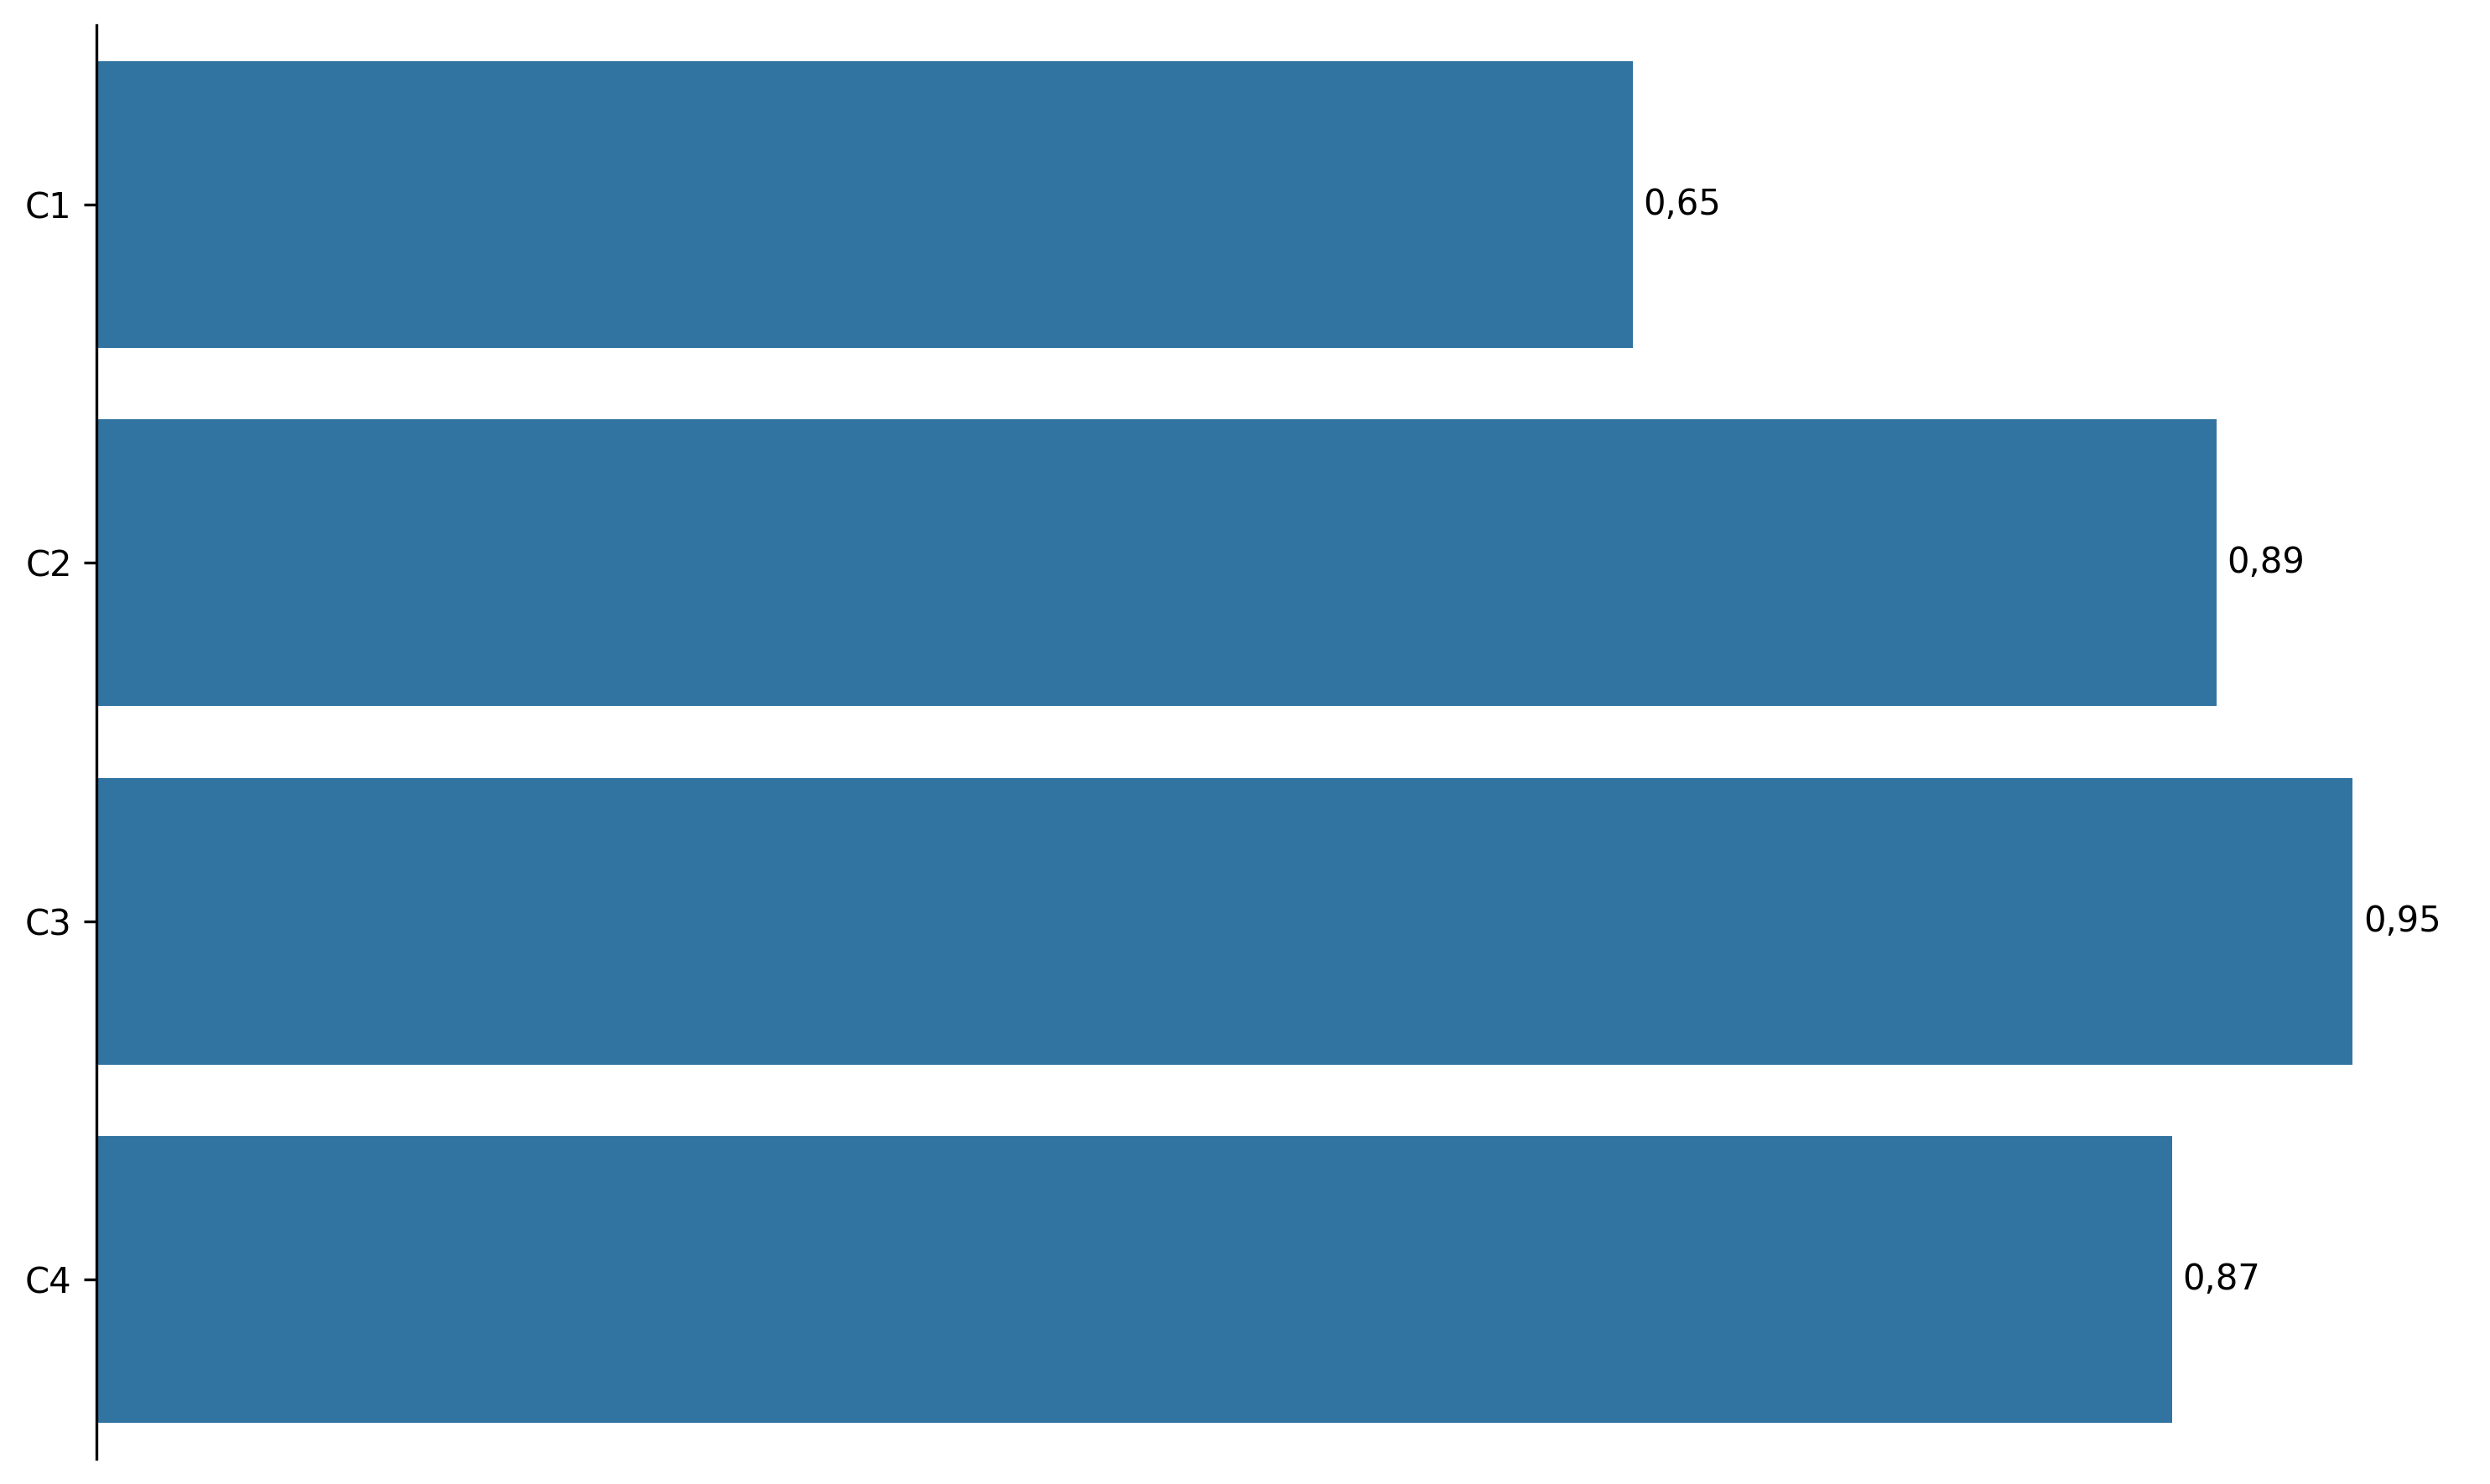
\includegraphics[width=1\linewidth]{figuras/comparacao_democracia.png}
	\label{fig:comparacao_democracia}
	\footnotesize{Fonte: elaboração própria baseada em \cite{rule-of-law-index}, \cite{jus_constraints_on_gov}, \cite{judicial-corruption-score} e \cite{human-rights-index-vdem}.}
\end{figure}

Nota-se da figura \ref{fig:comparacao_democracia} que a relação índice de democracia eleitoral x índice de corrupção judiciária tem uma correlação positiva média, enquanto as relações dos índices de controle judicial sob o Poder Executivo, liberdade civil e de Estado de Direito com o índice de democracia eleitoral tem correlações positivas fortes. Ou seja, controle judicial sob o Poder Executivo, liberdade civil e de Estado de Direito têm grande impacto na democracia. 

Considerando a análise de coeficiente de correlação anterior, destaque-se que o Brasil está em posição privilegiada, pois, se apenas 25\% dos 193 países alcançaram uma pontuação superior e metade alcançou menos que a média mundial, isso é um indicativo de que autocracias são prevalentes. \cite{nord2025democracy} informa que o Brasil, juntamente com o Equador, Lesoto e a Polônia, pararam e reverteram processos de autocratização antes da disrupção da democracia, exibindo resiliência a rupturas autocráticas.

Outros dados que reforçam a importância da democracia no Brasil foram apresentados por \cite{nord2025democracy} no relatório \textbf{Democracy Report 2025} da V-Dem relativo ao ano de 2024 na lista abaixo:

\begin{itemize}
    \item Democracias liberais representam menos de 12\% da população mundial, ou seja, menos de 900 milhões de pessoas.
    \item Democracias eleitorais representam 17\% da população mundial.
    \item 40\%  da população mundial - 3,1 bilhões de pessoas - vive em países que estão em processo de autocratização.
    \item Há mais autocracias do que democracias no mundo: 91 contra 88. Em 2023, era o contrário.
    \item O mundo tem apenas 29 liberais, o que torna o regime o mesmo comum.
    \item 72\% das pessoas no mundo vivem em autocracias, percentual mais alto desde 1978.
\end{itemize}

Dados internacionais confirma a real democracia do Brasil. \cite{rule-of-law-index} mostra na figura \ref{fig:key-features-of-liberal-democracy} como os índices de uma democracia liberal no Brasil são altos.

\begin{figure}[H]
	\centering
	\caption{Característica principal de democracia eleitoral no Brasil em 2024}
	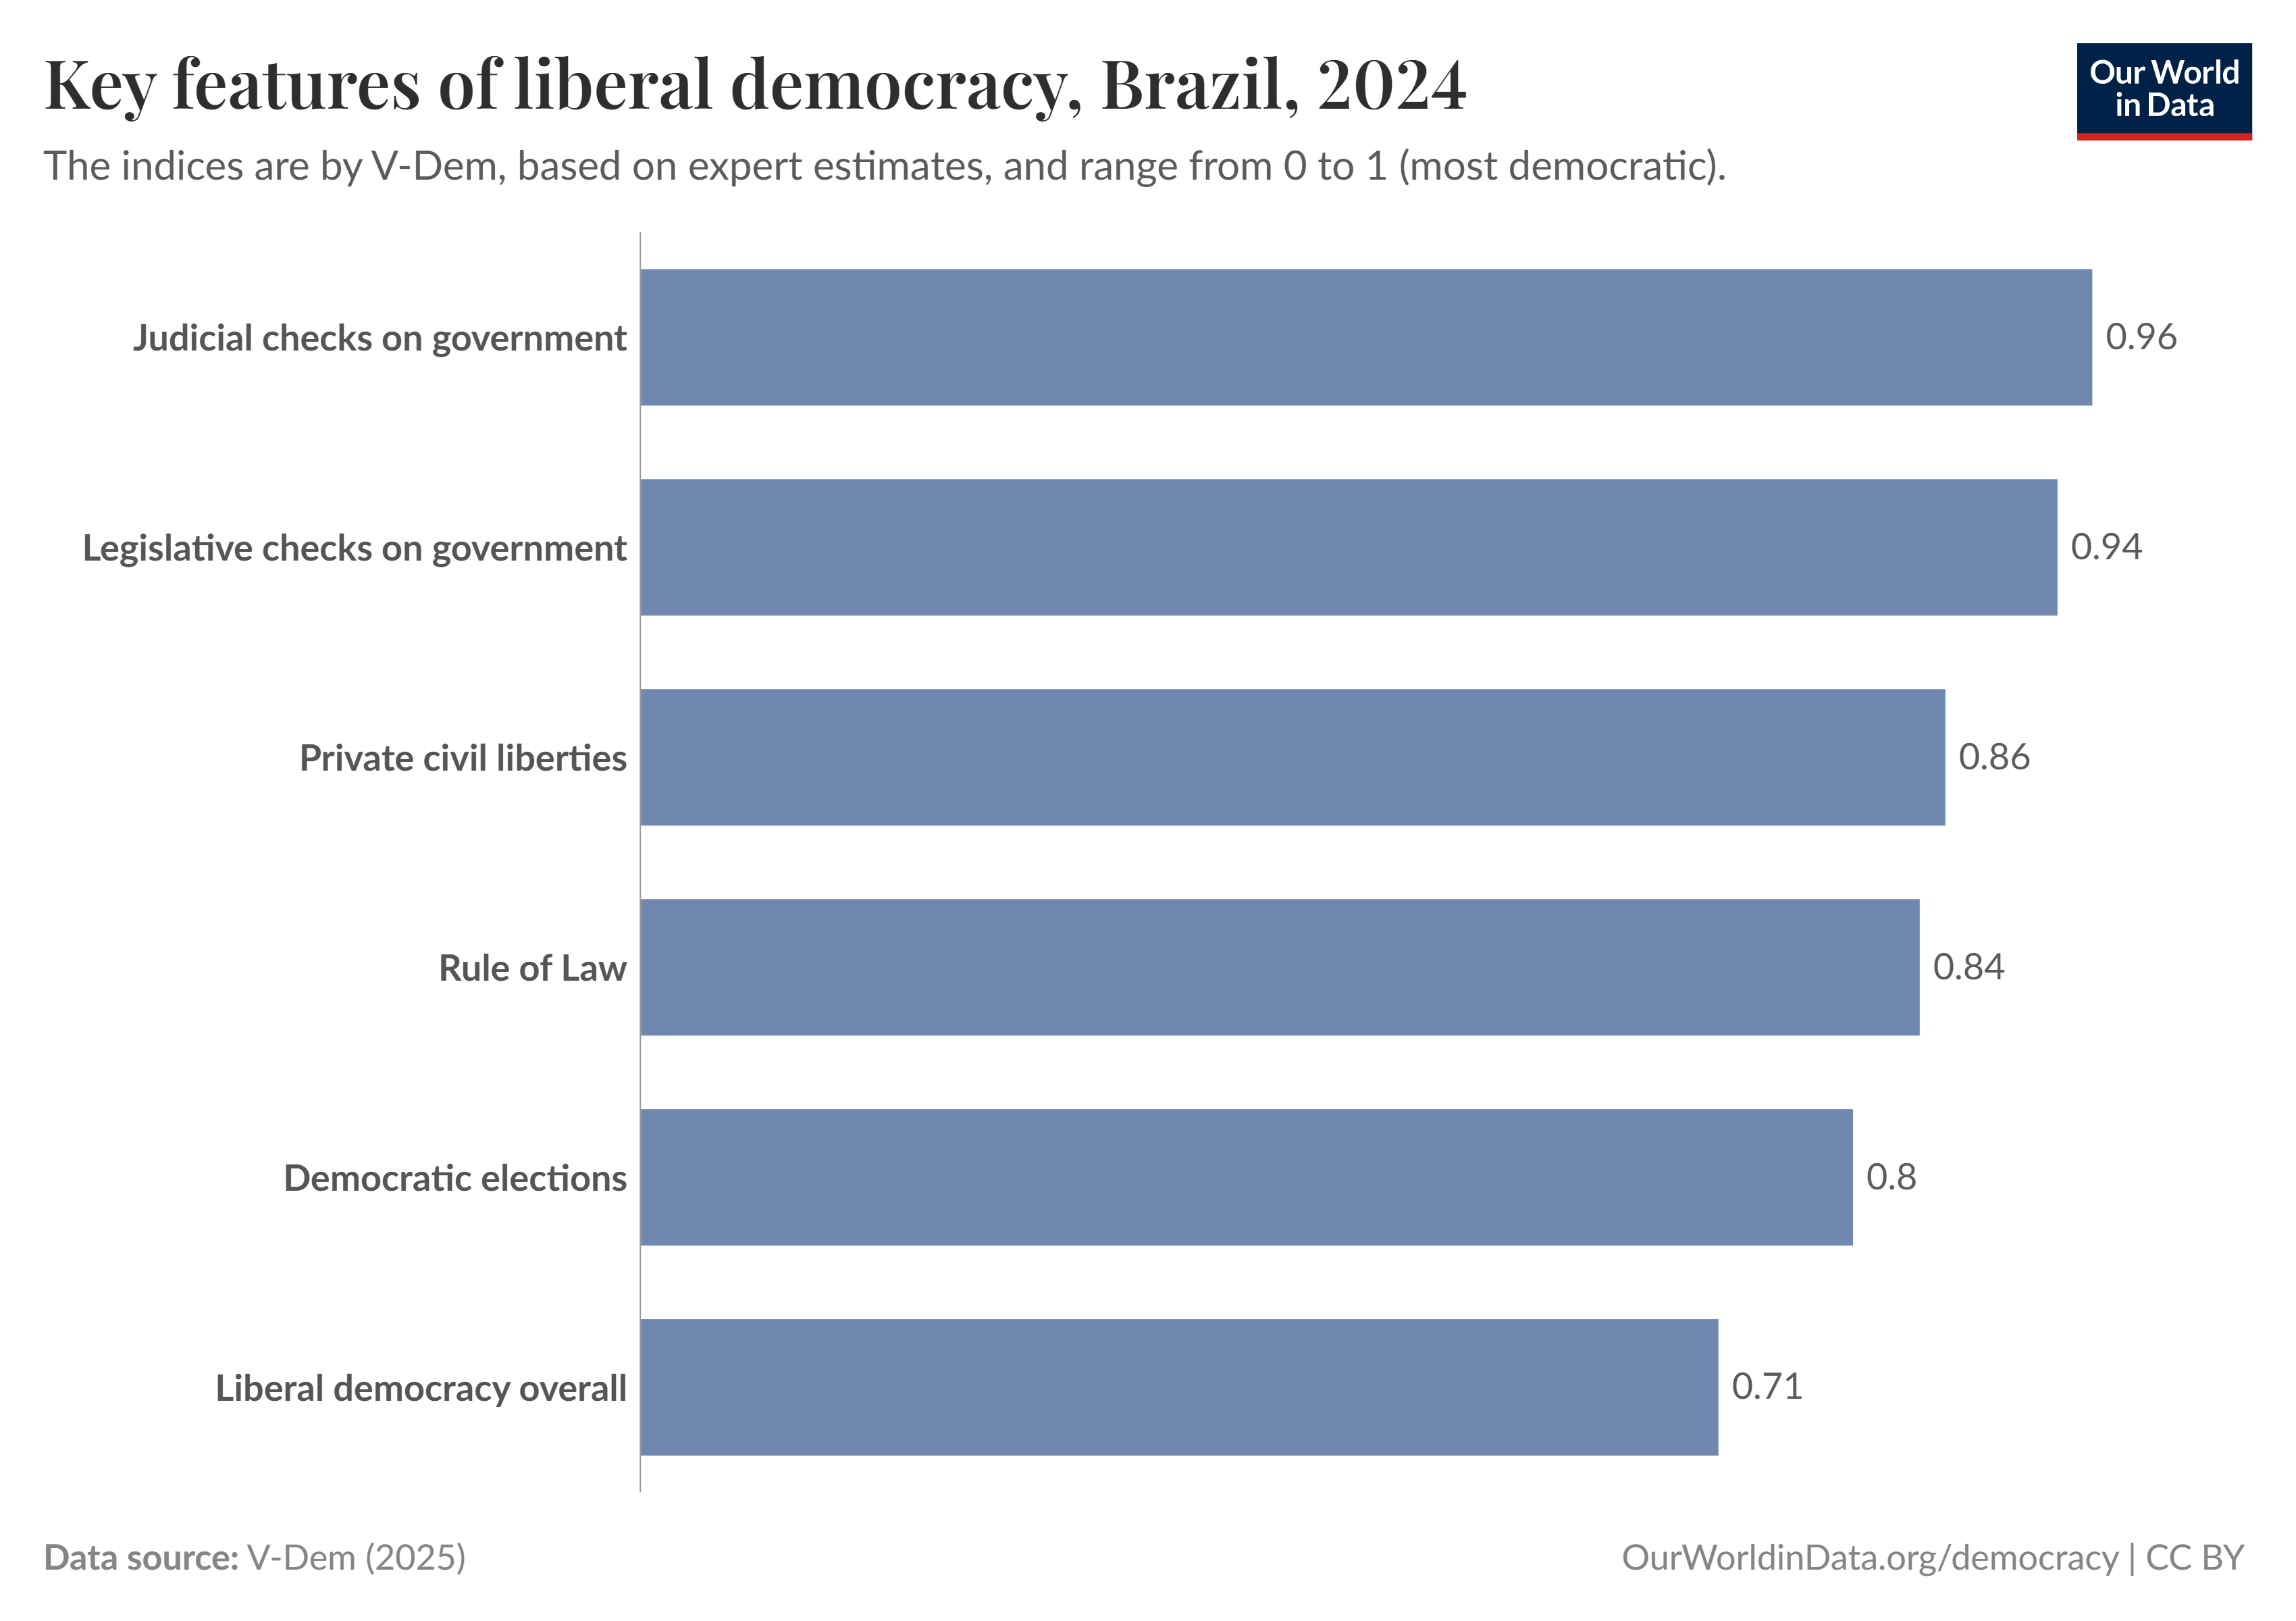
\includegraphics[width=1\linewidth]{figuras/key-features-of-liberal-democracy.png}
	\label{fig:key-features-of-liberal-democracy}
	\footnotesize{Fonte: \cite{rule-of-law-index}.}
\end{figure}

Como expresso pela figura \ref{fig:key-features-of-liberal-democracy}, além do controle judicial sobre o Poder Executivo e o Estado de Direito já citados em parágrafos anteriores, o controle legislativo sobre o Poder Executivo, as liberdades civis, as eleições democráticas são altas.

No tocante à liberdade de expressão e associação, bem como, as liberdades civis, a figura \ref{fig:comparacao_liberdade_expressao_associacao_dh}.
.
\begin{figure}[H]
	\centering
	\caption{Índice de liberdade de expressão, liberdade de associação e de liberdades civis no Brasil e a média mundial em 2024}
	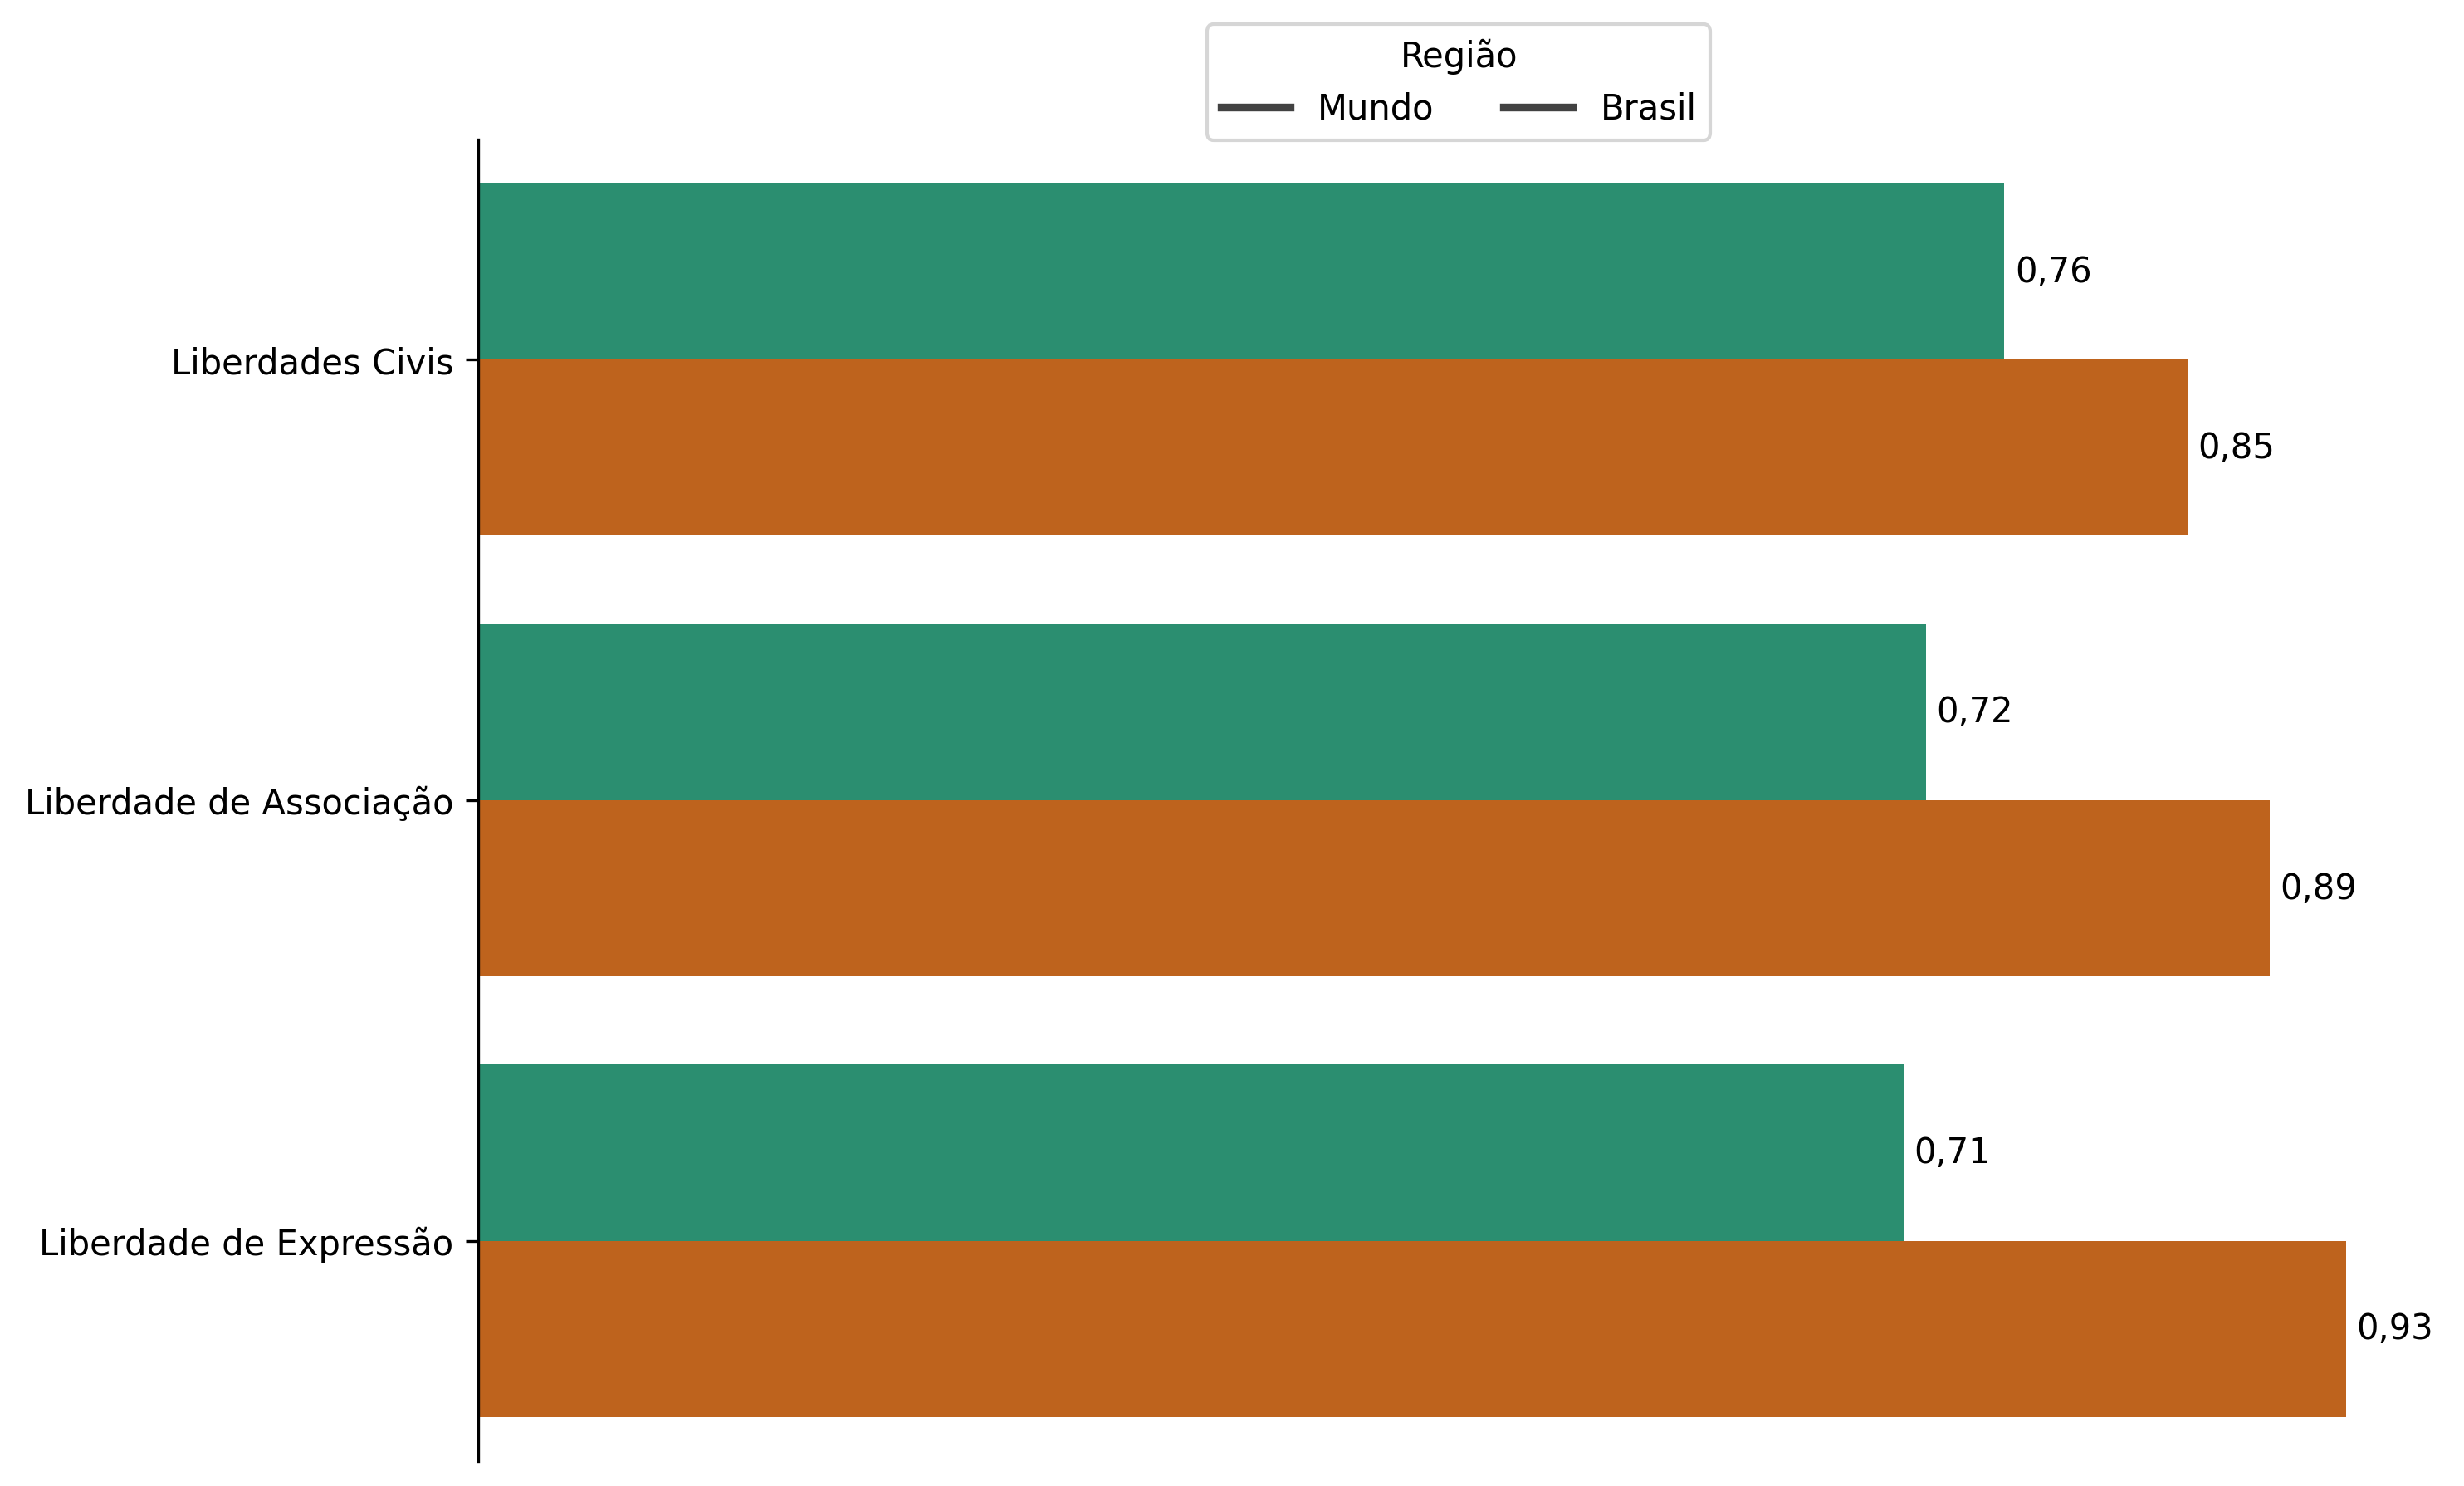
\includegraphics[width=1\linewidth]{figuras/comparacao_liberdade_expressao_associacao_dh.png}
	\label{fig:comparacao_liberdade_expressao_associacao_dh}
	\footnotesize{Fonte: elaboração própria baseada em \cite{freedom-of-association-index}, \cite{freedom-of-expression-index} e \cite{human-rights-index-vdem}.}
\end{figure}

Conforme expresso na figura \ref{fig:comparacao_liberdade_expressao_associacao_dh}, o Brasil se destaca nos quesitos liberdade de expressão e associação, bem como, os direitos humanos em relação à média mundial.

Os tópicos citados nas figuras \ref{fig:key-features-of-liberal-democracy} e \ref{fig:comparacao_liberdade_expressao_associacao_dh} representam temas ligados à Constituição Federal de 1988. Um exemplo é direito de associação, presente no art. 5º, XVII da Carta Magna, conforme \cite{cf88}, declara como plena a liberdade de associação para fins lícitos, vedada a de caráter paramilitar. O art. 37, VI, nos termos da Constituição, haja vista \cite{cf88}, garante ao servidor público civil o direito à livre associação sindical.

Outro exemplo é o do controle legislativo sobre o Poder Executivo. A Constituição Federal de 1988 concedeu ao Congresso Nacional, com auxilio do Tribunal de Contas da União, haja vista \cite{cf88}, poder fiscalizador sob o Poder Executivo via comissões permanentes, temporárias, especiais e as de inquérito parlamentar.

A Constituição Federal de 1988, assim argumentado por \cite{cf88}, concedeu competência constitucional para o Congresso Nacional sustar os atos normativos do Poder Executivo que exorbitem do poder regulamentar ou dos limites de delegação legislativa.

Ao Congresso Nacional, segundo \cite{cf88}, cabe sustar os efeitos jurídicos, respeitados os direitos adquiridos, de medidas provisórias expedidas pelo Presidente da Republica. E, por fim, conduzir a remoção do cargo de Presidente da República do seu ocupante.

As informações alarmantes apresentadas por \cite{nord2025democracy} expõem o quão benéfica tem sido a democracia para o Brasil desde a redemocratização. Embora o Brasil ainda apresente desafios, o país está em processo de melhoria institucional. Um exemplo disso é o fato do Brasil ter tido a capacidade de reverter uma tentativa de autocratização enquanto 40\%  da população mundial vive em países que estão em processo de autocratização.

Como consequência da argumentação anterior, \cite{pires2021paradoxo} corrobora a independência do Poder Judiciário. Para o autor, o Poder Judiciário obteve níveis elevados de independência com a Constituição Federal de 1988, que em um esforço para fortalecer a independência individual dos juízes, os termos e condições de mandato foram significativamente aprimorados.  Bem como, a Constituição Federal também fortaleceu a independência funcional do judiciário como instituição de governança, isolando-o do sistema político mais amplo.

No tocante aos direitos humanos, algumas decisões de caráter nacional foram aprovadas. Na ADPF 527, de acordo com \cite{adpf527}, "Assim, com base em diálogo institucional estabelecido com o Poder Executivo, como explicitado acima, ajusto os termos da cautelar já deferida para outorgar às transexuais e travestis com identidade de gênero feminina o direito de opção por cumprir pena: (i) em estabecimento prisional feminino; ou (ii) em estabelecimento prisional masculino, porém em área reservada, que garanta a sua segurança."

Outra decisão afeta aos direitos é a jurisprudência do Superior Tribunal de Justiça em relação a interpretação judicial e a aplicação do art. 318-A do Código de Processo Penal, introduzido pela Lei nº 13.769, de 2018, haja vista \cite{cpp}:

\noindent
\begin{flushleft}
\setlength{\leftskip}{4cm}
\small
"Art. 318-A.  A prisão preventiva imposta à mulher gestante ou que for mãe ou responsável por crianças ou pessoas com deficiência será substituída por prisão domiciliar, desde que: (Incluído pela Lei nº 13.769, de 2018).

I - não tenha cometido crime com violência ou grave ameaça a pessoa;              (Incluído pela Lei nº 13.769, de 2018).

II - não tenha cometido o crime contra seu filho ou dependente. (Incluído pela Lei nº 13.769, de 2018)." \cite{cpp}
\end{flushleft}

Visando a plena garantia dos direitos humanos por mulheres que são mães ou responsáveis legais, o Superior Tribunal de Justiça tem diversas decisões que usaram o art. 318-A do Código de Processo Penal. 

O RHC 145.931/MG, de 2021, aplicou o art. 318-A do Código de Processo Penal, cujo texto da ementa segue abaixo:

\noindent
\begin{flushleft}
\setlength{\leftskip}{4cm}
\small
"RECURSO EM HABEAS CORPUS. EXECUÇÃO PENAL.	EXECUÇÃO DE PENA PRIVATIVA DE LIBERDADE DE 9 ANOS DE RECLUSÃO. REGIME INICIAL FECHADO. CONDENAÇÃO PELA PRÁTICA DOS CRIMES DE TRÁFICO DE DROGAS E ASSOCIAÇÃO PARA O TRÁFICO. PRETENSÃO DE CONCESSÃO DE PRISÃO DOMICILIAR. PACIENTE GENITORA DE CRIANÇAS DE 6 E 2 ANOS DE IDADE. POSSIBILIDADE. CARACTERIZADA INEFICIÊNCIA ESTATAL EM DISPONIBILIZAR VAGA À RECORRENTE EM ESTABELECIMENTO PRISIONAL PRÓPRIO E ADEQUADO À SUA CONDIÇÃO PESSOAL, DOTADOS DE ASSISTÊNCIA MÉDICA PRÉ-NATAL E PÓS-PARTO, BERÇÁRIOS E CRECHES. ARTS. 82, § 1º, E 83, § 2º, DA LEP. PRESÍDIO FEMININO MAIS PRÓXIMOS DISTANTE 230 KM DA RESIDÊNCIA. CONVIVÊNCIA E AMAMENTAÇÃO IMPOSSIBILITADA. PROTEÇÃO INTEGRAL À CRIANÇA. PRIORIDADE. HC COLETIVO STF N. 143.641/SP. PRECEDENTES DO STJ. LIMINAR DEFERIDA. PARECER MINISTERIAL PELA CONCESSÃO DA ORDEM, EM MENOR EXTENSÃO, A FIM DE QUE A CORTE DE JUSTIÇA SEJA INSTADA A EXAMINAR O MÉRITO DO WRIT IMPETRADO NAQUELA INSTÂNCIA NO TOCANTE À TESE ALEGADA NA INICIAL DA AÇÃO MANDAMENTAL. ILEGALIDADE MANIFESTA 	EVIDENCIADA. RECURSO PROVIDO." \cite{rhc145931}
\end{flushleft}

Evidencia-se da análise da ementa que a mulher julgada foi está sendo condenada por tráfico de drogas e associação ao tráfico, porém na condição de genitora de duas crianças de 2 e 6 anos, foi-lhe concedida a possibilidade de responder em prisão domiciliar, conforme é demostrado abaixo:

\noindent
\begin{flushleft}
\setlength{\leftskip}{4cm}
\small
"2. Ademais, o CPP (com as alterações promovidas pela Lei nº 13.769/2018) passou a prever a substituição da prisão preventiva  por domiciliar à mulher gestante, mãe ou responsável por crianças ou pessoas com deficiência, desde que não tenha cometido crime com violência ou grave ameaça e o delito não tenha sido cometido o crime 	contra seu filho ou dependente, facultando, ainda, a aplicação de medidas cautelares (arts. 318-A e 318-B do CPP)." \cite{rhc145931}
\end{flushleft}

O posicionamento do Superior Tribunal foi reiterado por outra decisão, a Reclamação nº 40.676/SP.

\noindent
\begin{flushleft}
\setlength{\leftskip}{4cm}
\small
"1. A jurisprudência desta Corte tem se orientado no sentido de que deve ser dada uma interpretação extensiva tanto ao julgado proferido pelo Supremo Tribunal Federal no Habeas Corpus coletivo n. 143.641, que somente tratava de prisão preventiva de mulheres gestantes ou mães de crianças de até 12 anos, quanto ao art. 318-A do Código de Processo Penal, para autorizar também a concessão de prisão domiciliar às rés em execução provisória ou definitiva da pena, ainda que em regime fechado." \cite{reclamacao40676}
\end{flushleft}

Nota-se como a instância superior da Justiça Comum tem foco na dignidade da pessoas humana ao estabelecer como padrão de julgamento a aplicação plena do art. 318-A do Código de Processo Penal, focando na necessidade dos filhos e dependentes legais das mulheres rés na Justiça Criminal, concomitantemente, na condição de responsável e cuidadora de pessoas das rés de pessoas que delas dependem.

De forma complementar, o STF expediu em 2018 o HC nº 143.641/SP. De acordo com \cite{hc143641}, a determinação da Suprema Corte deu-se devido a reclamação das defensorias públicas dos Estados e da União de que as apenadas estavam sofrendo graves de violações dos direitos como gestantes e que seus filhos estariam sendo afetados por extensão, de modo que suas penas em unidades prisionais poderiam ser substituídas por penas alternativas, ou por estarem em prisão preventiva, seriam absorvidas depois. 
	
Outro fatores que motivaram a reclamação perante o Supremo Tribunal Federal, segundo \cite{hc143641}, foram as condições precárias das unidades prisionais que afetam tanto as apenadas, quanto sua prole. Adicionalmente, as apenas estavam tendo outros direitos que estão sendo desrespeitados, não se podendo penalizá-las pela falta de estrutura estatal adequada para fazê-los valer.

Complementarmente, haja vista \cite{hc143641}, foi argumentado que é o direito de punir, e não o direito à vida, à  integridade e à liberdade individual, que deve ser mitigado. Além disso, os reclamantes destacaram também a vulnerabilidade socioeconômica das mulheres presas preventivamente no Brasil. Requereram, por fim, a concessão da ordem para revogação da prisão preventiva decretada contra todas as gestantes puérperas e mães de crianças, ou sua substituição pela prisão domiciliar

Como resultado da independência proporcionada pela Constituição Federal, \cite{pires2021paradoxo} cita que os tribunais receberam controle total sobre seus assuntos administrativos, pessoais e disciplinares, de modo que o Poder Judiciário obteve controle quase total sobre seu orçamento.

No tocante à liberdade de expressão, \cite{daliberdade} cita que, na condição de um dos mais prestigiados direitos das sociedades democráticas, a liberdade de expressão encontra tutela na Constituição Federal, cujo art. 5º, inciso IV, dispõe que “é livre a manifestação do pensamento, sendo vedado o anonimato”.

Para \cite{daliberdade}, o direito à liberdade de expressão, que possui destacada função na concretização do Estado Democrático, em muitas situações se revela em rota de colisão com outros direitos de mesma hierarquia constitucional, principalmente quando está em jogo a delimitação da sua amplitude. 

Nesse sentido, em concordância com \cite{daliberdade}, Para a Corte Suprema, como visto, as linhas que autorizam restrições ao exercício da liberdade de expressão são bastante estreitas. Nesse contexto, o Tribunal não tem admitido proteção à liberdade de expressão em atos de incitação ao ódio, à intolerância e a violência, assim como tem vedado - para além do campo jurídico - manifestações que denotem conteúdo imoral, devendo, ainda, tal liberdade ser pautada pelo resguardo de outros direitos
fundamentais, como a honra, à intimidade e a privacidade.

Um exemplo da ação do Supremo Tribunal Federal foi a equiparação do crime de homofobia com o racismo, com base na Lei nº 7.716, de 1989. Conforme \cite{ado26}:

\noindent
\begin{flushleft}
\setlength{\leftskip}{4cm}
\small
"1. Até que sobrevenha lei emanada do Congresso Nacional destinada a
implementar os mandados de criminalização definidos nos incisos XLI e XLII do
art. 5º da Constituição da República, as condutas homofóbicas e transfóbicas, reais ou
supostas, que envolvem aversão odiosa à orientação sexual ou à identidade de gênero de
alguém, por traduzirem expressões de racismo, compreendido este em sua dimensão
social, ajustam-se, por identidade de razão e mediante adequação típica, aos preceitos
primários de incriminação definidos na Lei nº 7.716, de 08/01/1989, constituindo,
também, na hipótese de homicídio doloso, circunstância que o qualifica, por configurar motivo torpe (Código Penal, art. 121, § 2º, I, “in fine”);" \cite{ado26}
\end{flushleft}

Outra marco ligado à liberdade de impressa foi a declaração de não-recepção pela Constituição Federal de 1988 da Lei nº 5.250, de 1967 - conhecida como Lei da Impressa. O Supremo Tribunal Federal aprovou a ADPF 130/DF visando garantir a liberdade de impressa no Brasil. Segundo \cite{adpf130}:

\noindent
\begin{flushleft}
\setlength{\leftskip}{4cm}
\small
"Tirante, unicamente, as restrições que a Lei Fundamental de 1988 prevê para o 'estado de sítio' (art. 139), o Poder Público somente pode dispor sobre matérias lateral ou reflexamente de imprensa, respeitada sempre a ideia-força de que quem quer que seja tem o direito de dizer o que quer que seja. Logo, não cabe ao Estado, por qualquer dos seus órgãos, definir previamente o que pode ou o que não pode ser dito por indivíduos e jornalistas. As matérias reflexamente de imprensa, suscetíveis, portanto, de conformação legislativa, são as indicadas pela própria Constituição, tais como: direitos de resposta e de indenização, proporcionais ao agravo; proteção do sigilo da fonte ("quando necessário ao exercício profissional"); responsabilidade penal por calúnia, injúria e difamação; diversões e espetáculos
públicos; estabelecimento dos "meios legais que garantam à pessoa e à família a possibilidade de se defenderem de programas ou programações de rádio e televisão que contrariem o disposto no art. 221, bem como da propaganda de produtos, práticas e serviços que possam ser nocivos à saúde e ao meio ambiente" (inciso II do § 3º
do art. 220 da CF); independência e proteção remuneratória dos profissionais de imprensa como elementos de sua própria qualificação técnica (inciso XIII do art. 5º); participação do capital estrangeiro nas empresas de comunicação social (§ 4º do
art. 222 da CF); composição e funcionamento do Conselho de Comunicação Social (art. 224 da Constituição)." \cite{ado26}
\end{flushleft}

\cite{da2023cadernos} cita outras julgados do STF relativos à liberdade de expressão no periódico \textbf{Cadernos de Jurisprudência do Supremo Tribunal Federal: Concretizando Direitos Humanos} cuja temática é a \textbf{liberdade de expressão, democracia e novas tecnologias}, tais como o HC nº 82.424, o RE nº 511.961, as ADPF nº 187, 4.815, as ADI nº 5.122, 2.566, 4.451, por exemplo.

Como forma de evitar a ingerência do Poder Executivo, \cite{pires2021paradoxo} argumenta que a Constituição Federal estabeleceu o STF é o responsável pela elaboração do orçamento anual da Justiça Federal e pelo encaminhamento direto ao Congresso Nacional. Assim, limitou-se o poder do Governo Federal sob o Poder Judiciário. 

Outro autor destacou a importância da independência do Poder Judiciário foi \cite{akutsu2012dimensoes}. Para ele, a importância de um Poder Judiciário independente dos Poderes Executivo e Legislativo decorre da necessidade de salvaguarda da liberdade individual dos cidadãos, que podem recorrer ao Judiciário contra abusos de autoridades de quaisquer dos três poderes. 

Para \cite{akutsu2012dimensoes}, a independência do Poder Judiciário não deve constituir óbice do cumprimento dos princípios e às normas da Constituição Federal pelos juízes. Além de poder serem responsabilizados perante os cidadãos. 

Complementarmente, para \cite{akutsu2012dimensoes} no caso da premissa da independência dos juízes e tribunais não se concretize, o desempenho do Poder Judiciário pode ser afetado, uma vez que os juízes enfrentariam óbices para  proferir sentenças que desagradassem pessoas afetadas por suas decisões.

Como fortalecedor da independência do Poder Judiciário, e como demonstração constitucional de sua importância para o Brasil, em 2004 o Congresso Nacional aprovou a Emenda à Constituição nº 45, de 2004. \cite{ec45_2004} criou o CNJ, as Súmulas Vinculantes do STF, extinguiu os Tribunais de Alçada e determinou sua incorporação aos Tribunais de Justiça, além das outras medidas estabelecidas.

No contexto da mudança legislativa promovida pela  Emenda à Constituição nº 45, de 2004, a criação do CNJ, através da publicação da referida Emenda à Constituição, foi precedida e sucedida de diversas celeumas relaciona das à sua natureza, constitucionalidade, legitimidade e efetividade.

Para \cite{silva2013transparencia}, a criação do CNJ, promovida pela publicação da Emenda à Constituição nº 45, de 2004, foi precedida e sucedida de diversas celeumas relaciona das à sua natureza, constitucionalidade, legitimidade e efetividade.  

Ao CNJ, segundo \cite{silva2013transparencia}, foram concedidos importantes poderes para que o órgão, respondendo do constituinte derivado, respondendo pelo controle da atuação administrativa e financeira do Poder Judiciário. São competências do CNJ, conforme \cite{cf88}, no art. 103-B, §4º, \textit{ipsi litteris}:

\noindent
\begin{flushleft}
	\setlength{\leftskip}{4cm}
	\small
	“§ 4º Compete ao Conselho o controle da atuação administrativa e financeira do Poder Judiciário e do cumprimento dos deveres funcionais dos juízes, cabendo-lhe, além de outras atribuições que lhe forem conferidas pelo Estatuto da Magistratura:
	
	I - zelar pela autonomia do Poder Judiciário e pelo cumprimento do Estatuto da Magistratura, podendo expedir atos regulamentares, no âmbito de sua competência, ou recomendar providências;
	
	II - zelar pela observância do art. 37 e apreciar, de ofício ou mediante provocação, a legalidade dos atos administrativos praticados por membros ou órgãos do Poder Judiciário, podendo desconstituí-los, revê-los ou fixar prazo para que se adotem as providências necessárias ao exato cumprimento da lei, sem prejuízo da competência do Tribunal de Contas da União;
	
	III - receber e conhecer das reclamações contra membros ou órgãos do Poder Judiciário, inclusive contra seus serviços auxiliares, serventias e órgãos prestadores de serviços notariais e de registro que atuem por delegação do poder público ou oficializados, sem prejuízo da competência disciplinar e correicional dos tribunais, podendo avocar processos disciplinares em curso, determinar a remoção ou à disponibilidade e aplicar outras sanções administrativas, assegurada ampla defesa;
	
	IV - representar ao Ministério Público, no caso de crime contra a administração pública ou de abuso de autoridade;
	
	V - rever, de ofício ou mediante provocação, os processos disciplinares de juízes e membros de tribunais julgados há menos de um ano;
	
	VI - elaborar semestralmente relatório estatístico sobre processos e sentenças prolatadas, por unidade da Federação, nos diferentes órgãos do Poder Judiciário;
	
	VII - elaborar relatório anual, propondo as providências que julgar necessárias, sobre a situação do Poder Judiciário no País e as atividades do Conselho, o qual deve integrar mensagem do Presidente do Supremo Tribunal Federal a ser remetida ao Congresso Nacional, por ocasião da abertura da sessão legislativa.”
\end{flushleft}         

As competências presentes no art. 103-B, §4º da Constituição Federal, atribuidas pelo Congresso Nacional, empoderam o CNJ como ordenador do Poder Judiciário . E como tal, o órgão tem modernizado o Poder Judiciário via seus atos administrativos. Consequentemente, serão analisados as políticas públicas de governo digital do Poder Judiciário Brasileiro aprovadas pelo CNJ, que modernizaram o poder judicante.

%Modernização do poder judiciário

%\section{Políticas públicas de governo digital no Judiciário}

%Creta

%Processo judicial eletrônico

%\Plataforma Digital do Poder Judiciário Brasileiro

%Justiça 4.0

%Justiça Aberta}

%DataJud

%https://www.cnj.jus.br/pesquisas-judiciarias/paineis-cnj/